\chapter{Base Experiment}
\label{ch:Base_Experiment}

This chapter describes the base experiment, which serves the purpose of applying the approach and probing the hypothesis, presented in Chapter \ref{ch:Methodology}. A summarized representation of the workflow can be seen in Fig. \ref{fig:base_workflow}. In the following, we outline the steps for executing the experiment and the results of the evaluation.

\begin{figure}[!htb]
  \centering
  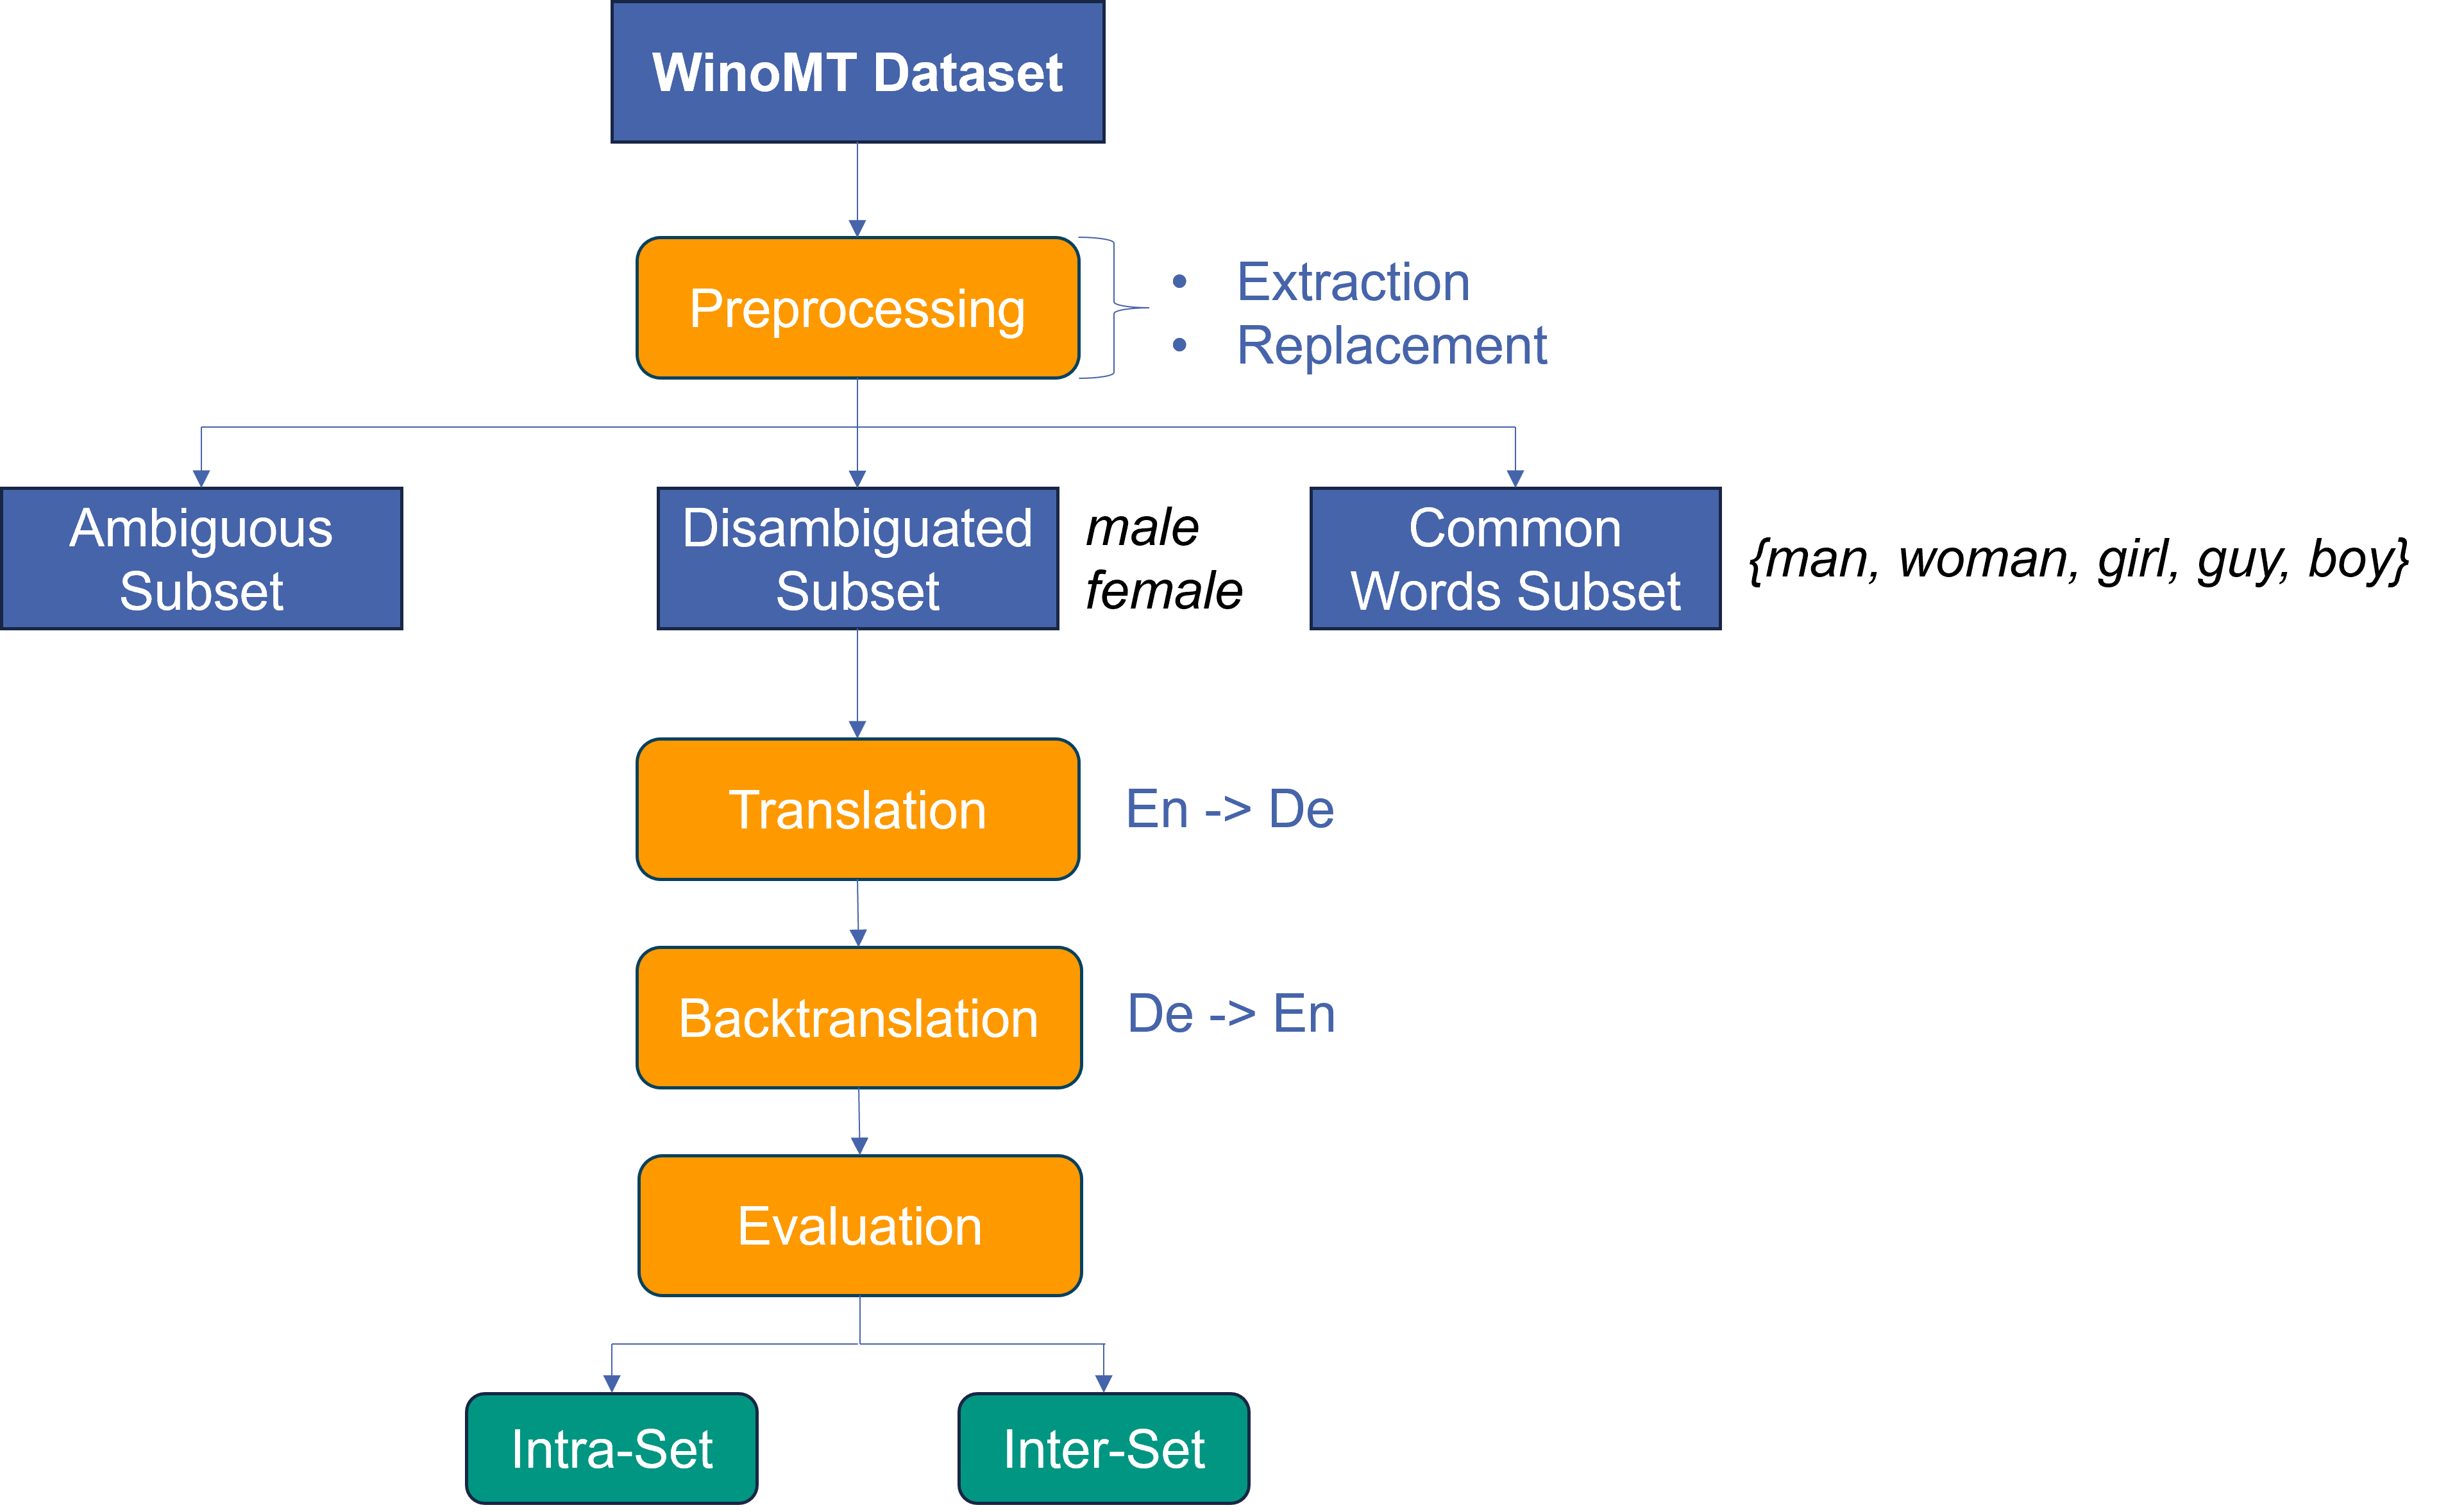
\includegraphics[scale=0.55]{figures/base_workflow.png}
  \caption{Base Experiment Workflow}
  \label{fig:base_workflow}
\end{figure}

%%%%%%%%%%%%%%%%%%%%%%%%%%%%%%%%%%%%%%%%%%%%%%%%%%%%%%%%%%%%%%%%%%%%%%%%%%%%%%%%%%%%%%%%%%%%
\section{Data Pre-processing}
\label{sec:Base_Experiment:Pre-processing}
The first step in conducting the base experiment is preprocessing the dataset. We use the artificially created WinoMT challenge set, presented in Subsection \ref{sec:Setup:Challenge_Set}. The sentences in this dataset usually consist of two gender-ambiguous occupation nouns and a context, containing disambiguation information about one of the occupations. We take the following steps to preprocess the sentences:

\begin{enumerate}
  \item \textbf{Sentence Extraction:}  
  In order to obtain fully ambiguous sentences, we remove the context information from the sentences and obtain a subset of 335 sentences from the type: "The developer argued with the designer.".
  To remove additional detection overhead, we want to have a single ambiguous word per sentence. For this purpose, we replace the second ambiguous word with a non-ambiguous proper noun, e.g., "John". 
  \item \textbf{Replacement:} As next, we generate new subsets of sentences, substituting the ambiguous word in the original sentence with a non-ambiguous version, using two different techniques:
  \begin{itemize}
      \item \textbf{Disambiguation:} We use the gender-defining adjectives \textit{male} and \textit{female} in front of the gender-ambiguous word. This technique is meant to force the translator to make the right decision regarding gender. % gender forcing
      \item \textbf{Common Words:} We replace the ambiguous word with each of the following common gender non-ambiguous words: \textit{man, woman, girl, guy, boy}. We evaluate for each word separately, as well as take the average of them. This method serves as a baseline for comparison against the disambiguated occupation nouns.
  \end{itemize}
\end{enumerate}

Table \ref{tab:preprocessing} shows the generated non-ambiguous subsets obtained by modifying the base ambiguous sentence "The developer argued with John.".

\begin{table}[!htb]
    \begin{tabularx}{\linewidth}{|l|X|l|}
        \hline
        \textbf{Replacement Method} & \textbf{Source Sentence} & \textbf{Source Word} \\ \hline
        \multirow{2}{*}{Disambiguation} & The \textbf{male developer} argued with John. & developer \\
        & The \textbf{female developer} argued with John. & developer \\ \hline
        \multirow{5}{*}{Common Words} & The \textbf{man} argued with John. & man \\
        & The \textbf{woman} argued with John. & woman \\
        & The \textbf{girl} argued with John. & girl \\
        & The \textbf{guy} argued with John. & guy \\
        & The \textbf{boy} argued with John. & boy \\ \hline
    \end{tabularx}
    \caption{\textbf{Example}: Non-ambiguous subsets for the baseline sentence "The developer argued with John.". \\ Source sentence: reflects the sentence in the non-ambiguous subset. \\ Source word: word in the sentence we evaluate for.}
    \label{tab:preprocessing}
\end{table}

The subsets resulting from the preprocessing are: 
\begin{itemize}
    \item \textbf{Ambiguous Subset}: a subset, containing the base ambiguous sentences.
    \item \textbf{Disambiguated Subset (male)}: a subset, containing the sentences, disambiguating the ambiguous word with \textit{male}.
    \item \textbf{Disambiguated Subset (female)}: a subset, containing the sentences, disambiguating the ambiguous word with \textit{female}.
    \item \textbf{Non-ambiguous Subsets}: five subsets, where the ambiguous word is replaced with the common words: \textit{man, woman, girl, guy, boy}.
\end{itemize}



%%%%%%%%%%%%%%%%%%%%%%%%%%%%%%%%%%%%%%%%%%%%%%%%%%%%%%%%%%%%%%%%%%%%%%%%%%%%%%%%%%%%%%%%%%%%
\section{Translation}
\label{sec:Base_Experiment:Translation}

The next step in conducting the experiments is translating the subsets of sentences. We translate from English to German. This is executed in two steps:

\begin{enumerate}
    \item \textbf{Translation Source -> Target:} 
    First, the subsets are translated in the target language (German).
    \item \textbf{Backtranslation Target -> Source:}
    The second step involves translating the translations back into the source language (English).
\end{enumerate}

For the purpose of  translation, we use two different decoding algorithms: Beam search and Sampling (see Subsection \ref{sec:Background:Decoding}). With Beam search, we compare the results for two different beam sizes: 10 and 100. The nbest size is the size of the number of unique translations, generated at each step. 

%%%%%%%%%%%%%%%%%%%%%%%%%%%%%%%%%%%%%%%%%%%%%%%%%%%%%%%%%%%%%%%%%%%%%%%%%%%%%%%%%%%%%%%%%%%%
\section{Word alignment}
\label{sec:Base_Experiment:Alignment}

In order to assign the words in the source sentence to their counterparts in the translations, we use two different alignment methods:

\begin{itemize}
    \item Source-to-translation (\textit{fast\_align}, \textit{awesome-align}): This alignment method aligns from the source language to the target language.
    \item Translation-to-translation (\textit{Tercom}): This alignment method aligns between two translations.
\end{itemize}

We use the first method to map each word in the source sentence to its translations and backtranslations in the target nbest lists. We do this in a two-step way, depicted in Fig. \ref{fig:alignment}. First, we align between the source sentence and the sentences in the nbest translations and extract the translations for each word. Then, we align between the translations and the backtranslations and extract the corresponding backtranslations resulting from the aligned translations of each word. 

We use the results from the second method as a baseline for comparison with the first method and to detect possible errors, which may occur in the information transfer between the two steps in the first method.

\begin{figure}[!htb]
  \centering
  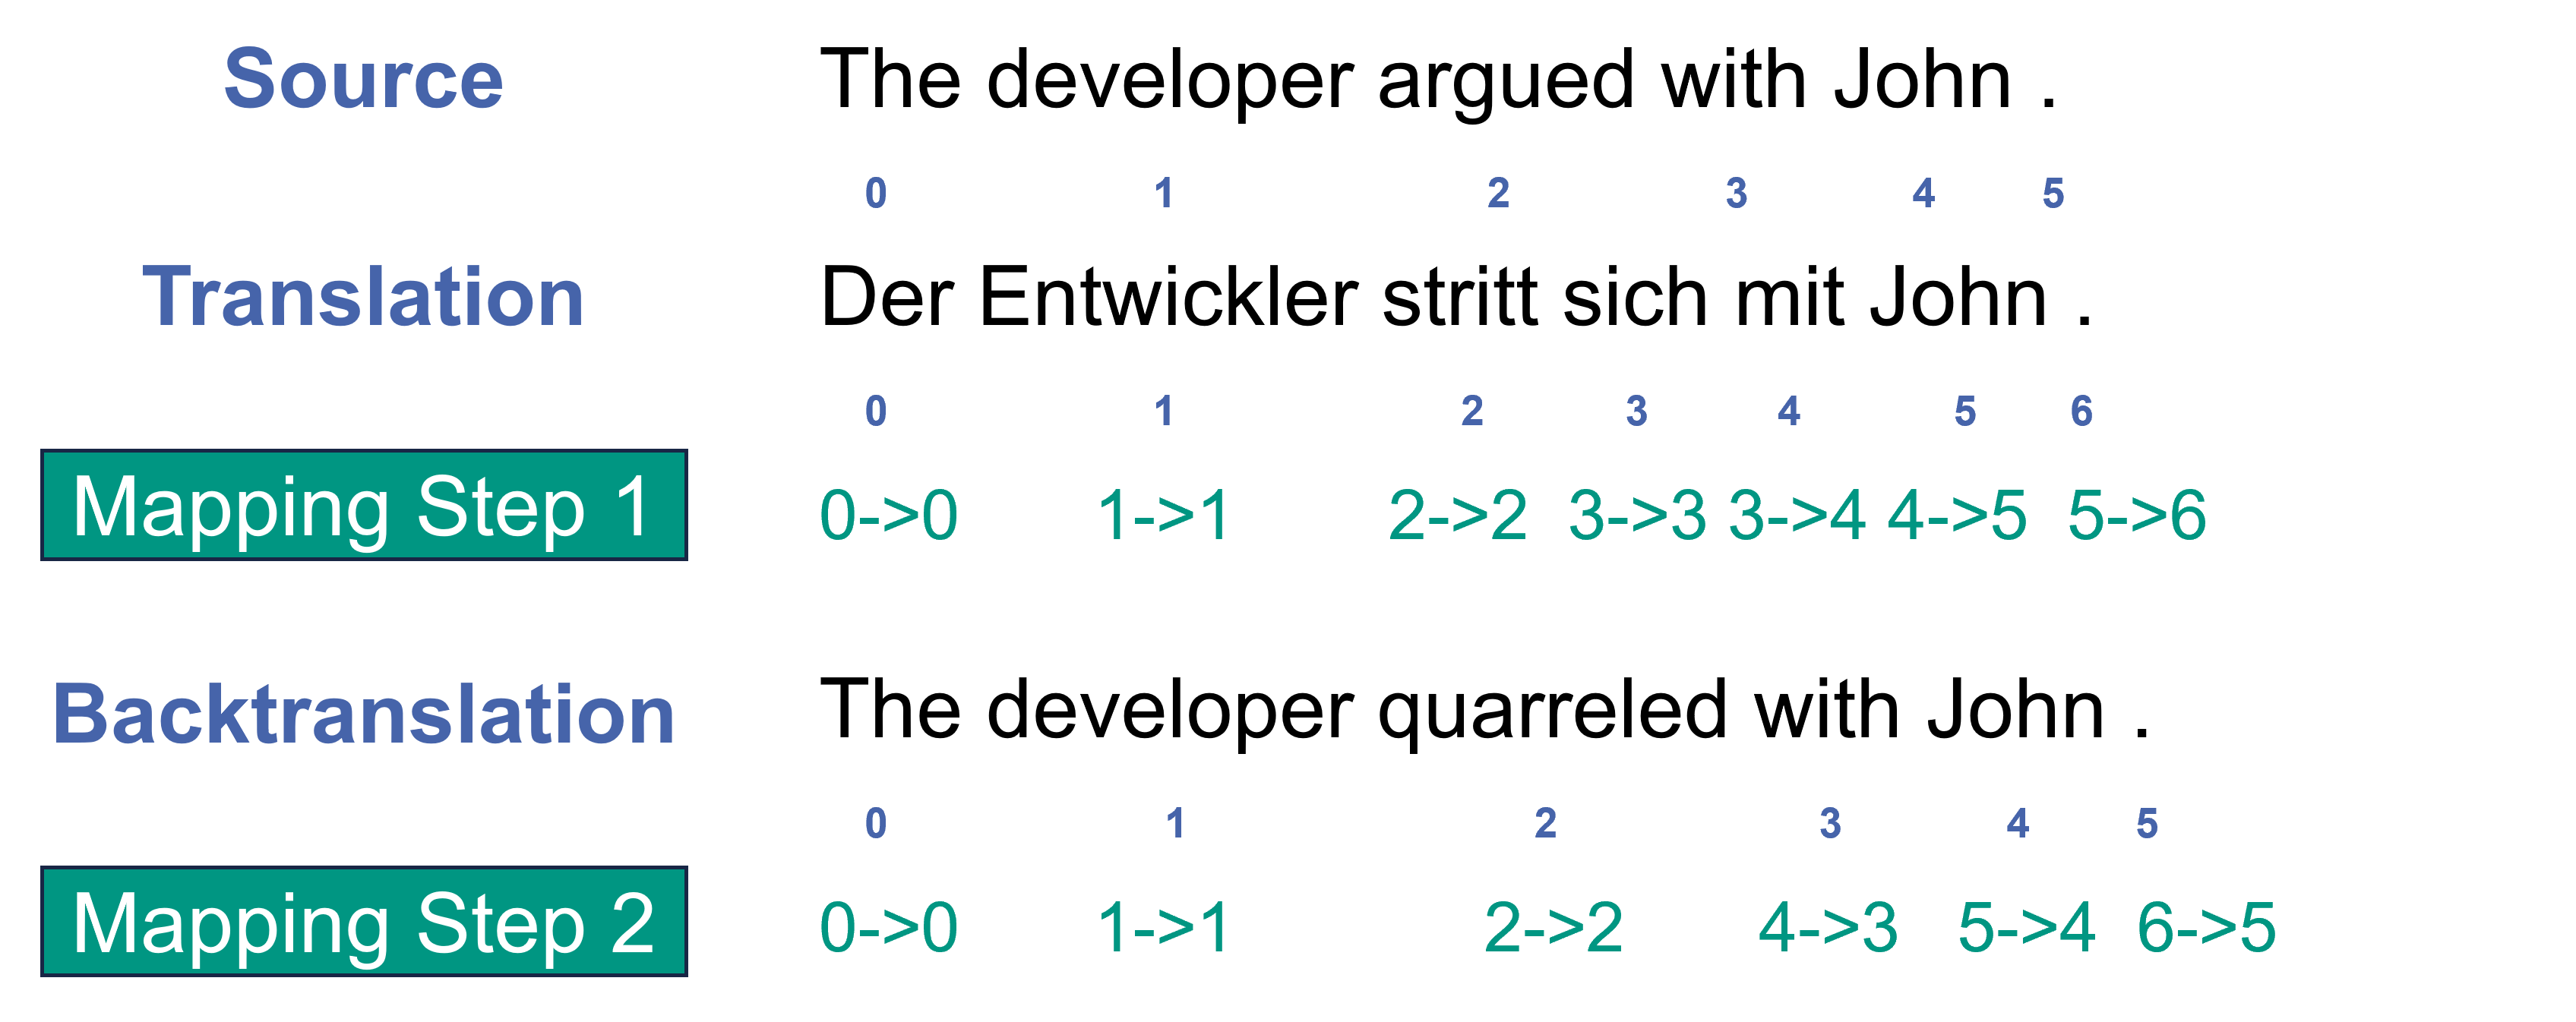
\includegraphics[scale=0.5]{figures/alignment.png}
  \caption{Example Illustration: 2-step mapping from source to translation and backtranslation}
  \label{fig:alignment}
\end{figure}

%%%%%%%%%%%%%%%%%%%%%%%%%%%%%%%%%%%%%%%%%%%%%%%%%%%%%%%%%%%%%%%%%%%%%%%%%%%%%%%%%%%%%%%%%%%%
\section{Evaluation}
\label{sec:Base_Experiment:Evaluation}

The last step in the experiments involves evaluating the translations and backtranslations to detect patterns using different statistical methods. These methods aim to probe the initial Hypothesis \ref{main}, discussed in Section \ref{sec:Methodology:Approach}. We apply all methods to all subsets, as presented in Section \ref{sec:Base_Experiment:Pre-processing}, and extract diversity information regarding the subsets themselves, as well as compare the results of the subsets against each other.

% define formally, maybe as a formula, pseudocode ???

%%%%%%%%%%%%%%%%%%%%%%%%%%%%%%%%%%%%%%%%%%%%%%%%%
\subsection{Reoccurrence Evaluation}
\label{sec:Base_Experiment:Statistics:Reoccurrence}
We evaluate how many of the source sentences and source words reoccur in the backtranslations:

\begin{enumerate}
    \item[1. ] Gather the backtranslations for each source sentences.
    \item[2a. ] Count the number of source sentences that reappear in their list of backtranslations.
    \item[2b. ] Count the number of source sentences which contain the source word in their backtranslations.
\end{enumerate}

% Is it to test which disambiguation method is better?
The purpose of this evaluation is to determine which of the subsets are able to reconstruct more of the source sentences/words. This could indicate which disambiguation method does better in restoring the original sentence. 

We also evaluate how often the source sentences and source words reoccur in the backtranslations:

\begin{enumerate}
    \item[1. ] Gather the backtranslations for each source sentences.
    \item[2a. ] Count in how many of the backtranslations the source sentences reappear.
    \item[2b. ] Count in how many of the backtranslations the source word reappears.
\end{enumerate}

We use this method to probe the Hypotheses \ref{d}. 

%%%%%%%%%%%%%%%%%%%%%%%%%%%%%%%%%%%%%%%%%%%%%%%%%
\subsection{Uniqueness Evaluation}
\label{sec:Base_Experiment:Statistics:Uniqueness}
We evaluate the number of unique words and sentences in the translations and backtranslations for each sentence of the subsets. 

For the sake of the evaluation, we follow this routine (\textit{[translations | backtranslations]} denotes that we follow the same step for both the translations and backtranslations):
\begin{enumerate}
    \item[1. ] Collect the \textit{[translations | backtranslations]} for each source sentences.
    % sentence level
    \item[2a. ] Count how many of the \textit{[translations | backtranslations]} are unique. 
    % word level
    \item[2b. ] Count how many unique words there are in the \textit{[translations | backtranslations]} and normalize the number by the total amount of words. 
    \item[3. ] Average the result for all sentences.
\end{enumerate}

We use this method to probe the Hypotheses \ref{a} and \ref{b}. 

%%%%%%%%%%%%%%%%%%%%%%%%%%%%%%%%%%%%%%%%%%%%%%%%%
\subsection{Gender Evaluation}
\label{sec:Base_Experiment:Statistics:Gender}
We perform the evaluation of gender on the translations of the subsets.  First, we align each word in the source sentence with its corresponding word in the translations and backtranslations (see Subsection \ref{sec:Base_Experiment:Alignment} for more detail). Then, we perform the following steps:

\begin{enumerate}
    \item[1. ] Gather the translations of the source word for each source sentence.
    \item[2. ] Detect the gender of the translations for each source sentence.
    \item[3a. ] Determine the proportion of source sentences producing \textit{male} versus \textit{female}.
    \item[3b. ] Calculate how many of the source sentences produce \textit{both genders}. 
\end{enumerate}

The purpose of this method is to assess if the translations produce the right gender (in the non-ambiguous subsets) or both genders (in the ambiguous subset) and how often they produce both genders for each subset.

%%%%%%%%%%%%%%%%%%%%%%%%%%%%%%%%%%%%%%%%%%%%%%%%%
\subsection{Alignment Evaluation}
\label{sec:Base_Experiment:Statistics:Alignment}
Another form of evaluation is based on the alignment of the words between the source sentence, the translations and backtranslations (see Subsection \ref{sec:Base_Experiment:Alignment} for more detail).

In order to assess the translations and backtranslations of the \textbf{source word}, we do:
\begin{enumerate}
    \item[1. ] Collect all \textit{[translations | backtranslations]} of the source word.
    \item[2. ] Count how many of the \textit{[translations | backtranslations]} are unique.
    \item[3. ] Average the result for all sentences.
\end{enumerate}

Similarly, to assess the translations and backtranslations of the \textbf{rest of the sentence} excluding the source word, we do:
\begin{enumerate}
    \item[1. ] Collect all \textit{[translations | backtranslations]} of the sentence rest.
    \item[2. ] Count how many of the \textit{[translations | backtranslations]} are unique.
    \item[3. ] Average the result for all sentences.
\end{enumerate}

The idea behind this evaluation method is to assess the Hypothesis \ref{c}.

Next, we will present the results of these statistical evaluations of the subsets.

%%%%%%%%%%%%%%%%%%%%%%%%%%%%%%%-----------------------------%%%%%%%%%%%%%%%%%%%%%%%%%%%%%%%%%%%%%%%
\section{Results}
\label{ch:Base_Experiment:Results}

% - Translation quality
% BLEU score on WinoMT: not possible, because no reference translations
% - Gender bias quality

We evaluate the translations and backtranslations of the different subsets based on the presented evaluation methods and present the results in the following subsections.

%%%%%%%%%%%%%%%%%%%%%%%%%%%%%%%%%%%%%%%%%%%%%%%%%
\subsection{Reoccurrence Evaluation Results}
\label{ch:Base_Experiment:Results:Reoccurrence}

\begin{table}[!htb] 
    \begin{subtable}{\textwidth}
        \centering
        \begin{tabularx}{\linewidth}{|X|XXXX|}
            \hline
             & \textbf{Ambiguous} & \textbf{Disambiguated (male)} & \textbf{Disambiguated (female)} & \textbf{Non-ambiguous average} \\ \hline
             \textbf{\#Sentences} & 295/335 & 293/335 & 118/335 & \underline{308/335} \\
             \textbf{\#Sentences (R)} & 295/335 & 6/335 & 25/335 & \underline{308/335} \\ 
             \textbf{Sentences } & 6.5/100 & 4.72/100 & 1.13/100 & \underline{6.69/100} \\ \hline
             \textbf{\#Words} & 329/335 & 330/335 & 314/335 & \underline{335/335} \\ 
             \textbf{\#Words (R)} & 329/335 & 330/335 & 314/335 & \underline{335/335} \\ 
             \textbf{Words} & 56.65/100 & 58.8/100 & 50.47/100 & \underline{71.26/100} \\ \hline
        \end{tabularx}
        \subcaption{\textbf{Beam search with beam size 10}. Backtranslation. Nbest size 10. Highest scores are underlined. \textbf{R}: removed German words for \textit{male} and \textit{female}. \\ First and second row: number of source sentences that reappear in the backtranslations. \\ Third row: averaged number of times the source sentences reoccur in 100 backtranslations. \\ Fourth and fifth row: number of source sentences which contain the source word in the backtranslations. \\ Sixth row: averaged number of times the source words reoccur in 100 backtranslations.}
        \label{tab:reoccurrence_10}
    \end{subtable}
    
    \begin{subtable}{\textwidth}
        \centering
        \begin{tabularx}{\linewidth}{|X|XXXX|}
            \hline
             & \textbf{Ambiguous} & \textbf{Disambiguated (male)} & \textbf{Disambiguated (female)} & \textbf{Non-ambiguous average} \\ \hline
             \textbf{\#Sentences} & 329/335 & \underline{330/335} & 281/335 & 329/335 \\ 
             \textbf{Sentences} & 72.51/10000 & 48.59/10000 & 21.85/10000 & \underline{70.94/10000} \\ \hline
             \textbf{\#Words} & 335/335 & 335/335 & 335/335 & 335/335 \\
             \textbf{Words} & 4714.74/10000 & 4788.99/10000 & 4192.54/10000 & \underline{5925.98/10000} \\ \hline
        \end{tabularx}
        \subcaption{\textbf{Beam search with beam size 100}. Backtranslation. Nbest size 100. Highest scores are underlined. \\ First row: number of source sentences that reappear in the backtranslations. \\ Second row:  averaged number of times the source sentences reoccur in 10000 backtranslations. \\ Third row: number of source sentences which contain the source word in the backtranslations. \\ Fourth row: averaged number of times the source words reoccur in 10000 backtranslations.}
        \label{tab:reoccurrence_100}
    \end{subtable}

    \begin{subtable}{\textwidth}
        \centering
        \begin{tabularx}{\linewidth}{|X|XXXX|}
            \hline
             & \textbf{Ambiguous} & \textbf{Disambiguated (male)} & \textbf{Disambiguated (female)} & \textbf{Non-ambiguous average} \\ \hline
             \textbf{\#Sentences} & 270/335 & 249/335 & 87/335 & \underline{295/335} \\ 
             \textbf{Sentences} & 3.99/100 & 2.52/100 & 0.58/100 & \underline{4.54/100} \\ \hline
             \textbf{\#Words} & 332/335 & 333/335 & 326/335 & \underline{335/335} \\
             \textbf{Words} & 50.83/100 & 49.02/100 & 43.86/100 & \underline{66.83/100} \\ \hline
        \end{tabularx}
        \subcaption{\textbf{Sampling}. Backtranslation. Nbest size 10. Highest scores are underlined. \\ First row: number of source sentences that reappear in the backtranslations. \\ Second row:  averaged number of times the source sentences reoccur in 100 backtranslations. \\ Third row: number of source sentences which contain the source word in the backtranslations. \\ Fourth row: averaged number of times the source words reoccur in 100 backtranslations.}
        \label{tab:reoccurrence_sampling}
    \end{subtable}
    
    \caption{Reoccurrence Evaluation Results}
    \label{tab:reoccurrence}
\end{table}

The results from the evaluation of reoccurrence are listed in Table \ref{tab:reoccurrence}.
% Highest score
As we can observe, the average from the subsets of common words dominates the highest score in both the recurring sentences and words. This is to be expected, because the words in these subsets are most generic and have the highest probability of being predicted, compared to the occupational words from the WinoMT sentences in the other three subsets. 

% Interesting findings
Most interestingly, the female-disambiaguated subset has the lowest score for reoccurring sentences. When investigating the results, we found some discrepancy between the way "female" and "male" are translated. The "female" prefix is very often lost in the backtranslation, which results in the backtranslated sentence being regarded as differing from the source sentence. In contrast, the "male" prefix is most often preserved, resulting in the same sentence in backtranslation. We illustrate this with the following examples:

\begin{itemize}
    \item \textbf{Source (EN):} The \textit{female} developer argued with John. \\
    \textbf{Translation (DE):} Die Entwicklerin argumentierte mit John. \\
    \textbf{Backtranslation (EN):} The developer argued with John.
    
    \item \textbf{Source (EN):} The \textit{male} developer argued with John. \\
    \textbf{Translation (DE):} Der \textit{männliche} Entwickler argumentierte mit John. \\
    \textbf{Backtranslation (EN):} The \textit{male} developer argued with John.
\end{itemize}

As we can see, the "male" prefix is translated to its corresponding word in German "männliche", while the "female" prefix is lost in the translation, but its meaning is reflected in the female gender of the German word for developer "Entwicklerin".

Also, both disambiguation subsets sometimes generate the opposite gender with the correct prefix, for example, "der \textit{weibliche} Entwickler" (the \textit{female} male developer) and "die \textit{männliche} Entwicklerin" (the \textit{male} female developer). This presents a contradiction that influences the translation quality. We tried mitigating this by removing the German words for "female" and "male" from the translations with Beam search with beam size 10 (see Table \ref{tab:reoccurrence_10}). As we can see, this has a significant effect on the reoccurrence in backtranslation for the disambiguated subsets. For the male-disambiguated subset, only 6 out of 335 sentences reoccur, while for the female-disambiguated subset 25 out of 335 sentences reoccur. The conclusion we can make from these results is that the gender prefix words "male" and "female" most often reappear in backtranslation, when they are initially translated to their German counterpart, and when this is not the case, they are less likely to be reproduced in backtranslation for male than for female.

We note that the findings from these results are important and will have an effect on the further experiments.

% Beam size 100
Table \ref{tab:reoccurrence_100} shows the results from the evaluation of reoccurrence for beam search with beam size 100. Here we can observe that more female sentences are reoccurring in backtranslation compared to beam 100, which means that increasing the beam increases the possibility for preservation of the "female" prefix in the backtranslations. Also, with beam size 100 the source word reappears for all source sentences in the backtranslations.

% Hypothesis d); Sampling
The results from Sampling, as seen in Table \ref{tab:reoccurrence_sampling}, show that the ambiguous word reoccurs more often in backtranslations than the corresponding disambiguated words (male and female), which was not the case with Beam search. Although the non-ambiguous word still reoccurs most often, this is a positive result for Hyp. \ref{d}.

%%%%%%%%%%%%%%%%%%%%%%%%%%%%%%%%%%%%%%%%%%%%%%%%%
\subsection{Uniqueness Evaluation Results}
\label{ch:Base_Experiment:Results:Uniqueness}

The results from the evaluation of uniqueness are listed in Table \ref{tab:uniqueness_translation} for translation and Table \ref{tab:uniqueness_backtranslation} for backtranslation.
Since we use the beam search algorithm for decoding with beam size 10 and nbest size 10, we expect it to generate 10 unique sentences per translation, which is almost always the case, as we see from the score for the number of unique sentences in translations. With Sampling, we sample a higher number of translations, and extract 10 unique translations from the generated samples.

% Table for Translation
\begin{table}[!htb]

    \begin{subtable}{\textwidth}
        \centering
        \begin{tabularx}{\linewidth}{|X|XXXX|}
            \hline
             & \textbf{Ambiguous} & \textbf{Disambiguated (male)} & \textbf{Disambiguated (female)} & \textbf{Non-ambiguous average} \\ \hline
             \textbf{Sentences} & 9.94/10 & 9.95/10 & 9.87/10 & \underline{9.97/10} \\ 
             \textbf{Words} & \underline{0.205} & 0.19 & 0.201 & 0.202 \\ \hline
        \end{tabularx}
        \caption{\textbf{Beam search with beam size 10}. Nbest size 10. Highest scores are underlined. \\ First row: Averaged number of unique sentences per source sentence out of 10 translations. \\ Second row: Averaged number of unique words per source sentence, normalized by the average total number of words in 10 translations.}
        \label{tab:uniqueness_translation_10}
    \end{subtable}

    \begin{subtable}{\textwidth}
        \centering
        \begin{tabularx}{\linewidth}{|X|XXXX|}
            \hline
             & \textbf{Ambiguous} & \textbf{Disambiguated (male)} & \textbf{Disambiguated (female)} & \textbf{Non-ambiguous average} \\ \hline
             \textbf{Sentences} & 10/10 & 10/10 & 10/10 & 10/10 \\ 
             \textbf{Words} & 0.278 & 0.277 & \underline{0.29} & 0.263 \\ \hline
        \end{tabularx}
        \caption{\textbf{Sampling}. Nbest size 10. Highest scores are underlined. \\ First row: Averaged number of unique sentences per source sentence out of 10 translations. \\ Second row: Averaged number of unique words per source sentence, normalized by the average total number of words in 10 translations.}
        \label{tab:uniqueness_translation_sampling}
    \end{subtable}
    \caption{\textbf{Uniqueness Evaluation Results for Translation}}
    \label{tab:uniqueness_translation}
\end{table}

% Table for Backtranslation
\begin{table}[!htb] 

    \begin{subtable}{\textwidth}
        \centering
        \begin{tabularx}{\linewidth}{|X|XXXX|}
            \hline
             & \textbf{Ambiguous} & \textbf{Disambiguated (male)} & \textbf{Disambiguated (female)} & \textbf{Non-ambiguous average} \\ \hline
             \textbf{Sentences} & 45.98/100 & 50.73/100 & \underline{50.82/100} & 47.06/100 \\
             \textbf{Sentences (R)} & 45.98/100 & 41.36/100 & 47.03/100 & \underline{47.06/100} \\ \hline
             \textbf{Words} & 0.044 & 0.039 & 0.043 & \underline{0.045} \\ 
             \textbf{Words (R)} & 0.044 & 0.042 & 0.043 & \underline{0.045} \\ \hline
        \end{tabularx}
        \caption{\textbf{Beam search with beam size 10}. Nbest size 10. \\ Highest scores are underlined. \textbf{R}: removed German words for \textit{male} and \textit{female}. \\ First and second row: Averaged number of unique sentences per source sentence out of 10 translations. \\ Third and fourth row: Averaged number of unique words per source sentence, normalized by the average total number of words in 100 backtranslations.}    
        \label{tab:uniqueness_backtranslation_10}
    \end{subtable}

    \begin{subtable}{\textwidth}
        \centering
        \begin{tabularx}{\linewidth}{|X|XXXX|}
            \hline
             & \textbf{Ambiguous} & \textbf{Disambiguated (male)} & \textbf{Disambiguated (female)} & \textbf{Non-ambiguous average} \\ \hline
             \textbf{Sentences} & 3181.51/10000 & 3391.55/10000 & \underline{3424.98/10000} & 3297.48/10000 \\ \hline
        \end{tabularx}
        \caption{\textbf{Beam search with beam size 100}. Nbest size 100. \\ Highest scores are underlined. Averaged number of unique sentences per source sentence out of 100 translations.}
        \label{tab:uniqueness_backtranslation_100}
    \end{subtable}

    \begin{subtable}{\textwidth}
        \centering
        \begin{tabularx}{\linewidth}{|X|XXXX|}
            \hline
             & \textbf{Ambiguous} & \textbf{Disambiguated (male)} & \textbf{Disambiguated (female)} & \textbf{Non-ambiguous average} \\ \hline
             \textbf{Sentences} & 81.81/100 & \underline{86.87/100} & 85.75/100 & 80.6/100 \\ 
             \textbf{Words} & 0.104 & 0.103 & \underline{0.108} & 0.098 \\ \hline
        \end{tabularx}
        \caption{\textbf{Sampling}. Nbest size 10. \\ Highest scores are underlined. \\ First row: Averaged number of unique sentences per source sentence out of 10 translations. \\ Third row: Averaged number of unique words per source sentence, normalized by the average total number of words in 100 backtranslations.}
        \label{tab:uniqueness_backtranslation_sampling}
    \end{subtable}

    \caption{\textbf{Uniqueness Evaluation Results for Backtranslation}}
    \label{tab:uniqueness_backtranslation}
\end{table}

%%% Range of uniqueness
\begin{figure}[!htb]
     \centering
     
     \begin{subfigure}{0.49\textwidth}
         \centering
         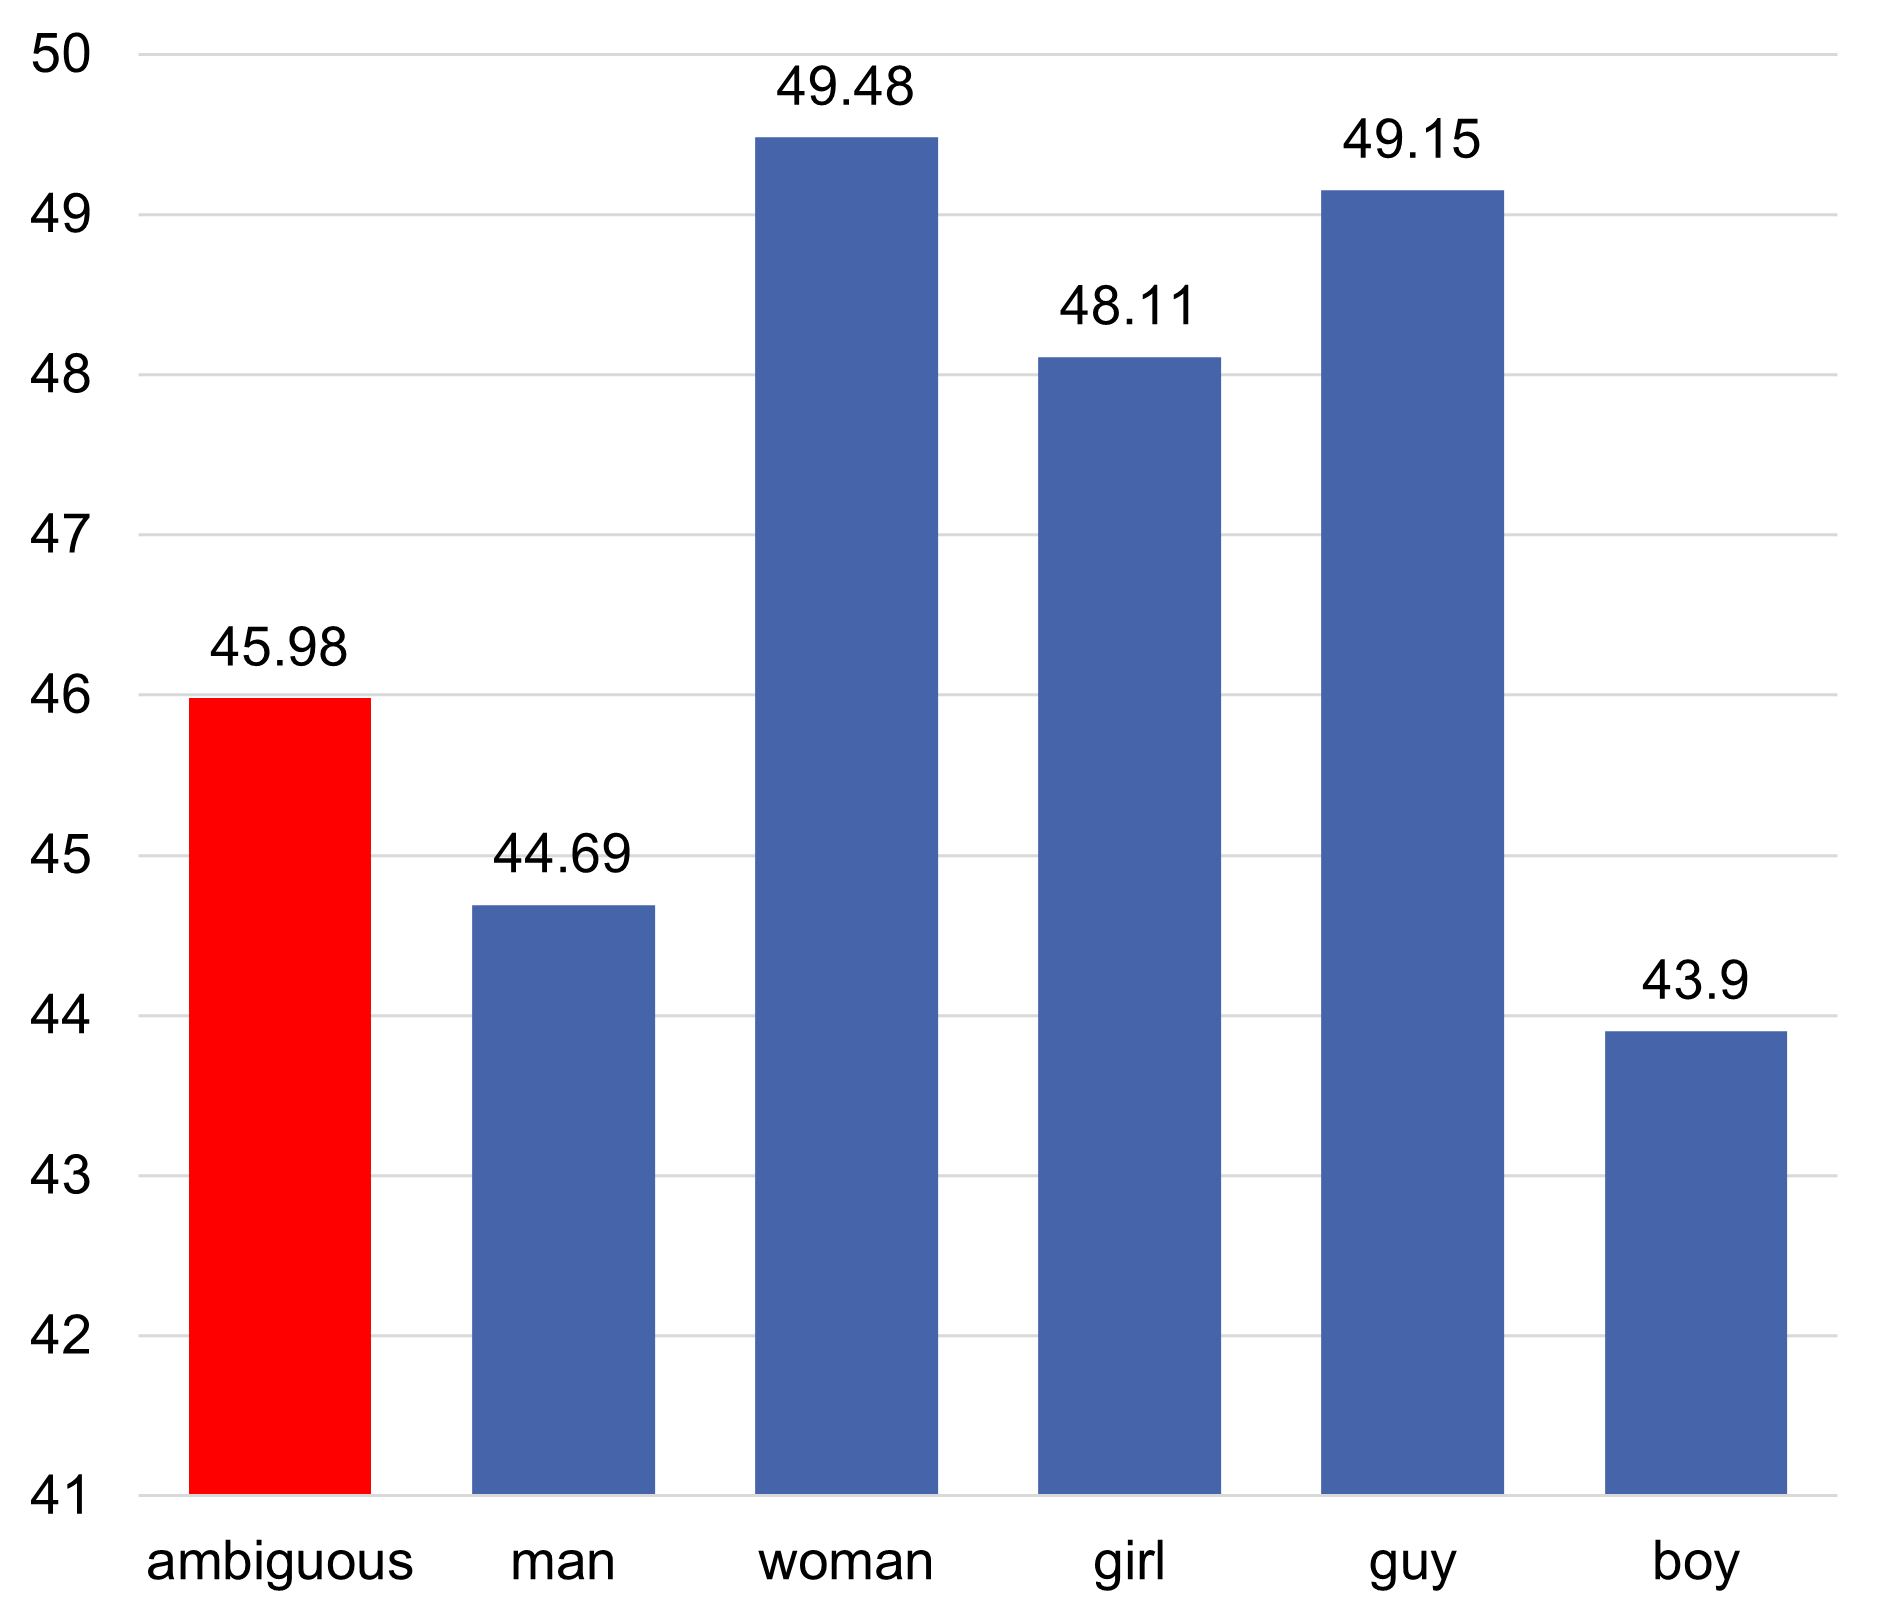
\includegraphics[width=\textwidth]{figures/uniqueness/range_beam_10.png}
         \caption{Beam search with beam size 10}
         \label{fig:uniqueness_range_10}
     \end{subfigure}
     \hfill
     \begin{subfigure}{0.49\textwidth}
         \centering
         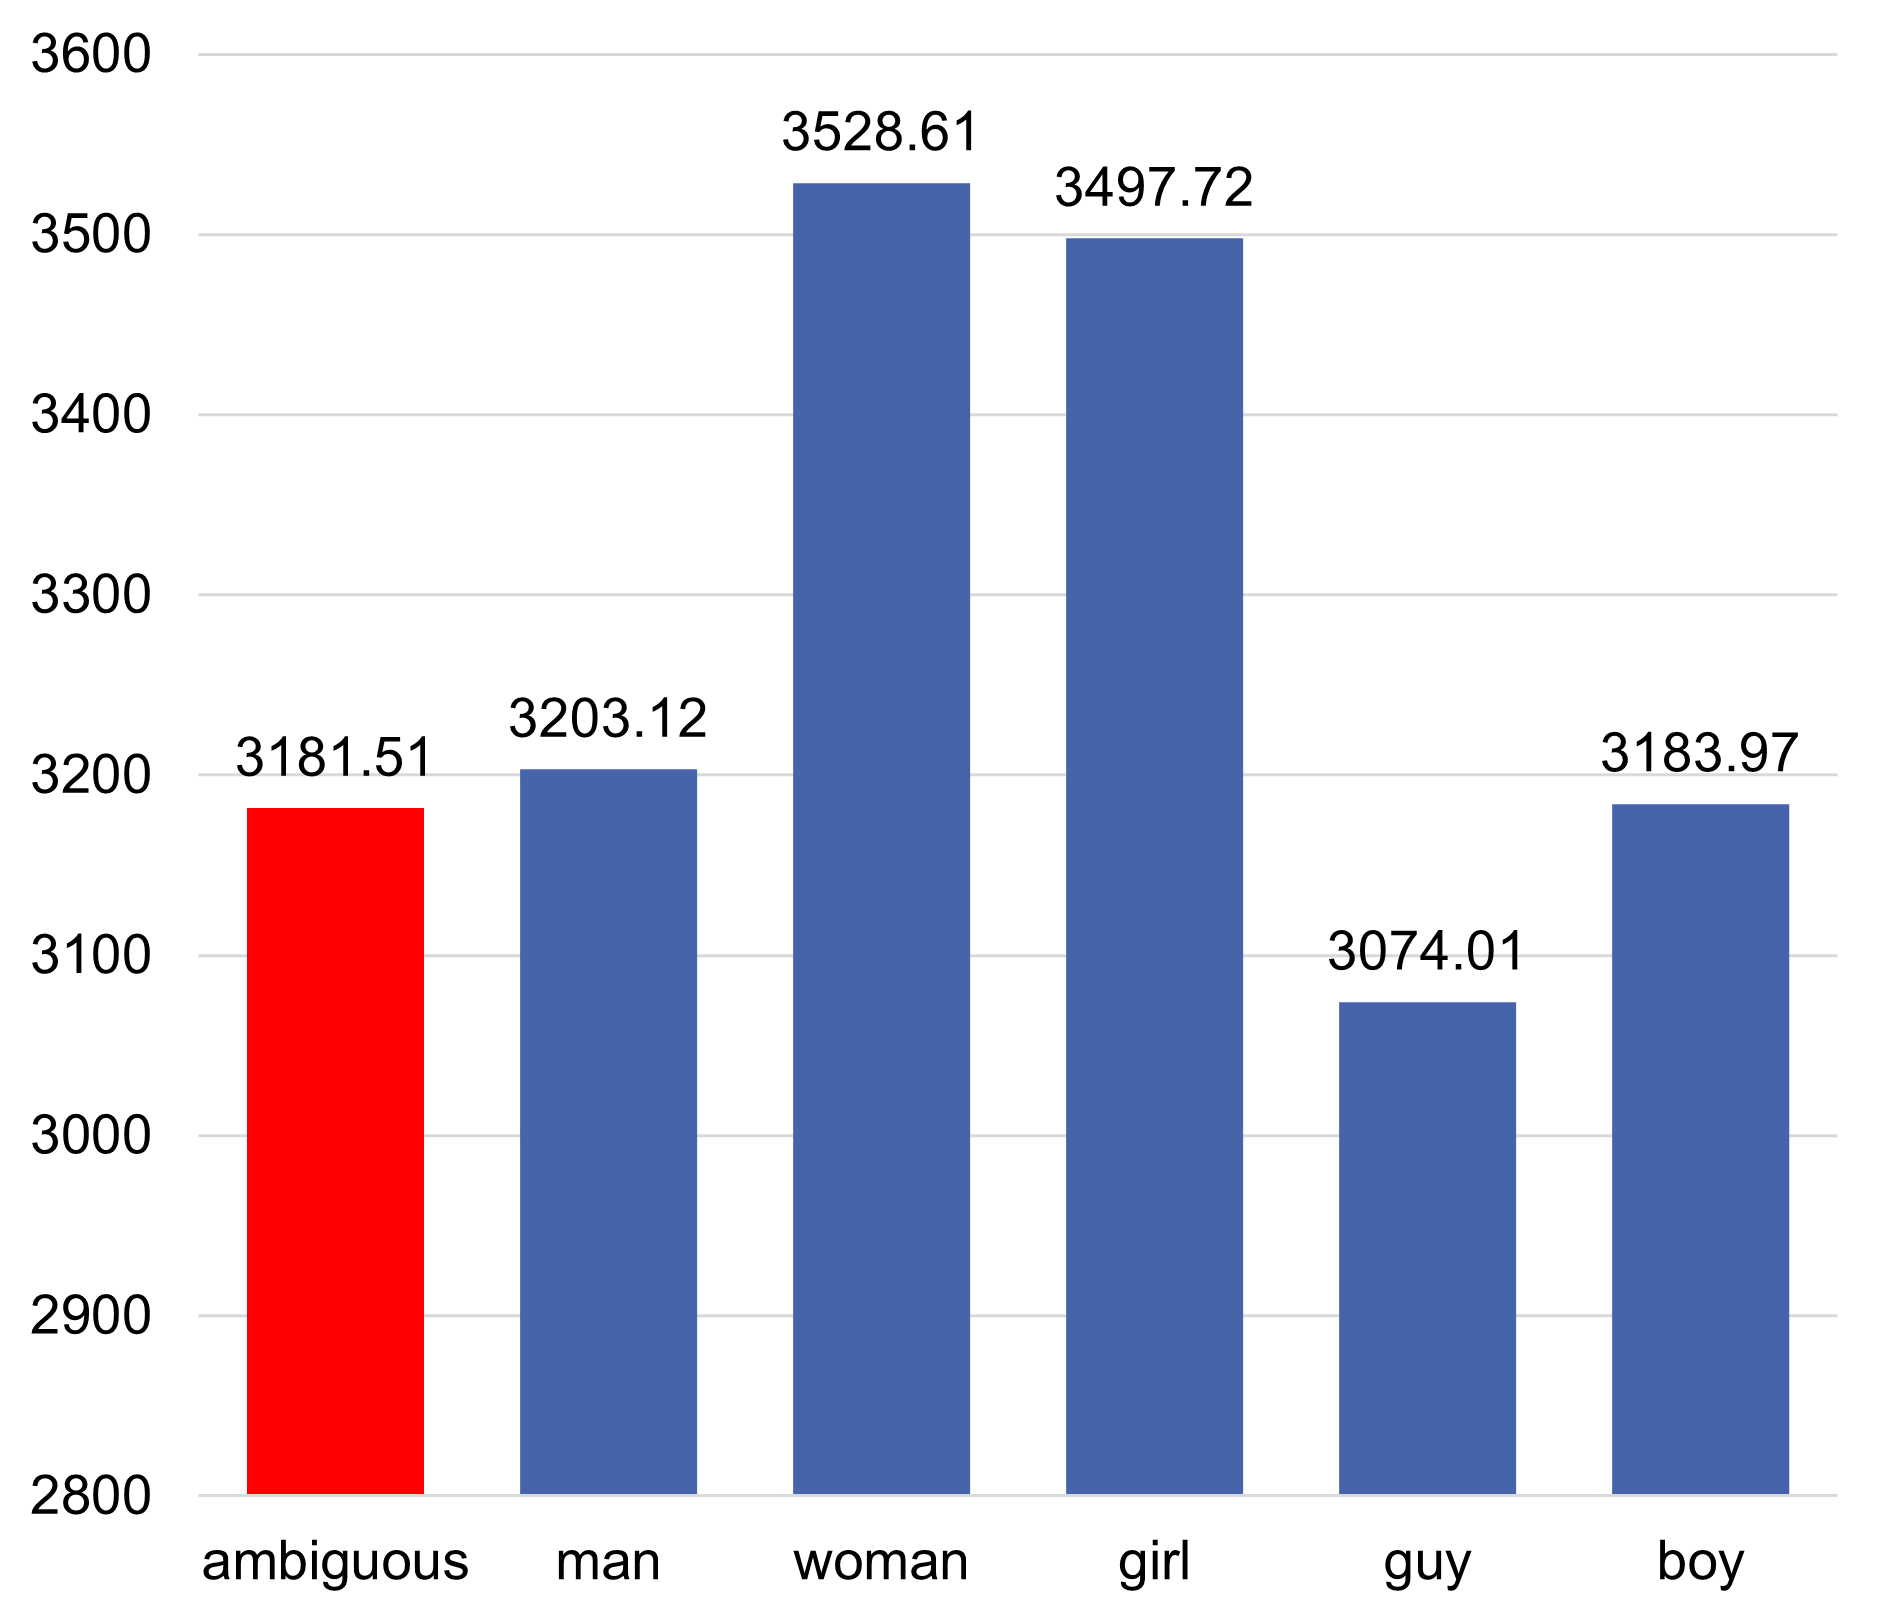
\includegraphics[width=\textwidth]{figures/uniqueness/range_beam_100.png}
         \caption{Beam search with beam size 100}
         \label{fig:uniqueness_range_100}
     \end{subfigure}
     
    \caption{Comparison Between the Number of Unique Backtranslations for Common Words and Ambiguous Subsets}
    \label{fig:uniqueness_range}

\end{figure}

% Graphs
\begin{figure}[!htb]
     \centering
     
     \begin{subfigure}{0.49\textwidth}
         \centering
         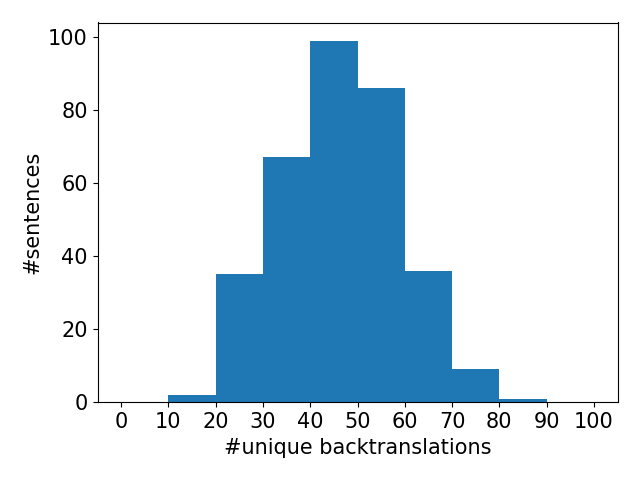
\includegraphics[width=\textwidth]{figures/uniqueness/unique_beam10/unique_back_original.png}
         \caption{Ambiguous Subset}
         \label{fig:uniqueness_ambiguous}
     \end{subfigure}
     \hfill
     \begin{subfigure}{0.49\textwidth}
         \centering
         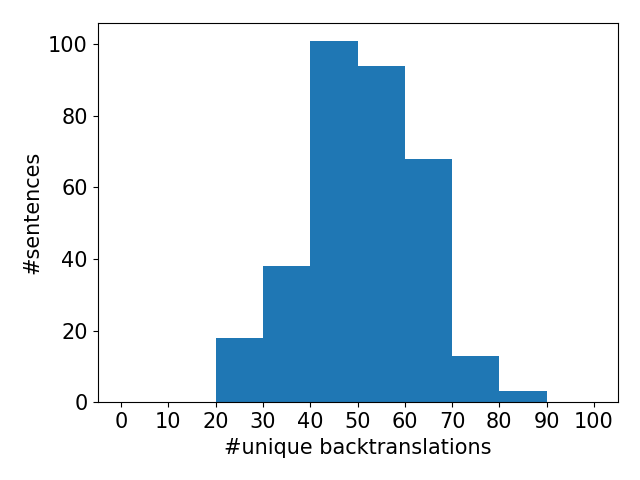
\includegraphics[width=\textwidth]{figures/uniqueness/unique_beam10/unique_back_male.png}
         \caption{Disambiguated Subset (male)}
         \label{fig:uniqueness_male}
     \end{subfigure}
     \begin{subfigure}{0.49\textwidth}
         \centering
         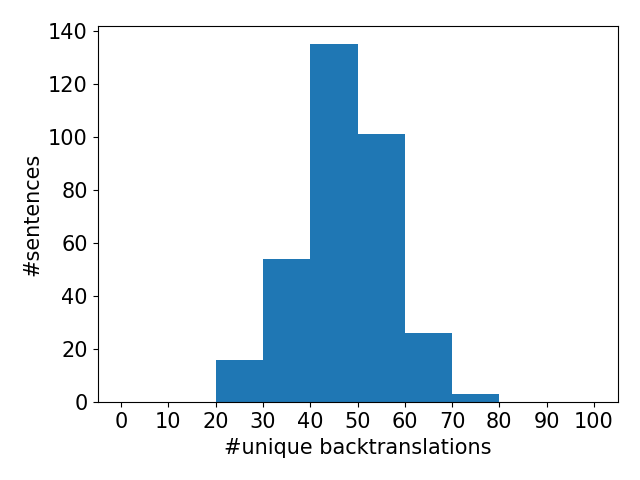
\includegraphics[width=\textwidth]{figures/uniqueness/unique_beam10/unique_back_average.png}
         \caption{Non-ambiguous Subset Average}
         \label{fig:uniqueness_common}
     \end{subfigure}
     \hfill
     \begin{subfigure}{0.49\textwidth}
         \centering
         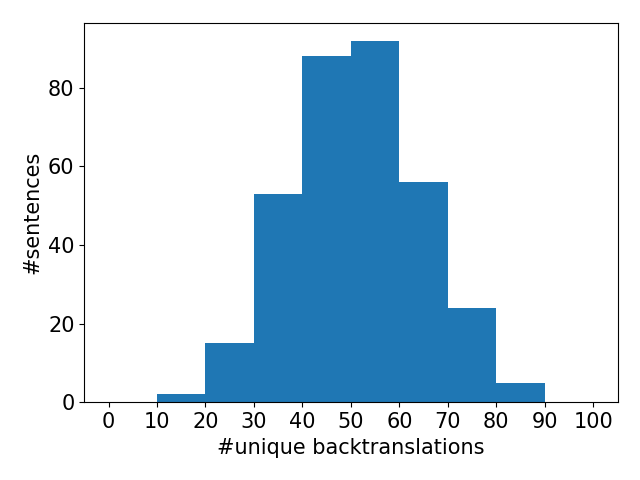
\includegraphics[width=\textwidth]{figures/uniqueness/unique_beam10/unique_back_female.png}
         \caption{Disambiguated Subset (female)}
         \label{fig:uniqueness_female}
     \end{subfigure}
        \caption{Distribution of Unique Backtranslations: Beam search with beam size 10}
        \label{fig:uniqueness_graphs_10}

\end{figure}

% Interesting findings
Most notable are the results for the number of unique backtranslations. As we can see in the first row of Table \ref{tab:alignment_backtranslation_10}, the ambiguous subset produces the least amount of unique sentences in backtranslation, which proves Hyp. \ref{a}. To inspect this further, we increase the beam size to 100, and as we see from Table \ref{tab:uniqueness_backtranslation_100} this experiment confirms the results.

However, when removing the German prefix gender words \textit{male} and \textit{female} we get mixed results in relation to the disambiguated subsets. The value for the male-disambiguation is the lowest, however the value for the ambiguous subset is still lower than the female-disambiguated subset. Then, we can speculate that modifying the translation in the suggested manner would not be further useful to the inspection of the approach.

% Range
To investigate this further, we regard the results for the different common words separately instead of averaged, as we can see in Fig. \ref{fig:uniqueness_range}. The minimum value in the range, 43.9 (for the word "boy") for beam size 10 and 3074.01 (for the word "guy") for beam size 100, is still lower for the common words compared to the ambiguous subset, 45.98 for beam size 10 and 3181.51 for beam size 100.

The results for the number of unique words in translation and backtranslation are inconclusive. Considering Hyp. \ref{b}, we expected the ambiguous subset to generate the least unique words in backtranslation, but this is not the case.

% Sampling
We also investigated the generated backtranslations from the Sampling method, as seen in \ref{tab:uniqueness_backtranslation_sampling}. Interestingly, Sampling generates almost twice as many unique backtranslations, reagrding both words and sentences. Here, the lowest score belongs to the non-ambiguous subset, contrary to the expectation from Hyp. \ref{a}. However, the ambiguous subset still has less unique backtranslations than the corresponding disambiguated subsets, which is what we expect.

% Distribution graphs
Furthermore, we plot the distribution of unique backtranslations, which can be seen in Fig. \ref{fig:uniqueness_graphs_10} for Beam search with beam size 10, containing the histograms for each subset. 
Most sentences have between 40 and 50 unique backtranslations , except for the female-disambiguated subset, which have between 50 and 60 unique backtranslations, confirming the highest score from Table \ref{tab:uniqueness_backtranslation}. Another observation we can make pertains to the difference between the ambiguous subset \ref{fig:uniqueness_ambiguous} and the non-ambiguous subset averaged for the common words (\ref{fig:uniqueness_common}). There, we can see that the range is smaller ([20, 80]) and more of the non-ambiguous sentences have the average amount of unique backtranslations (around 140 sentences), while the ambiguous sentences produce more variable amount of backtranslations in terms of range  ([10, 90]) but less amount of sentences producing the average amount of unique backtranslations (around 100 sentences).
The distribution of unique backtranslations for Beam search with beam size 100 and Sampling show the same trend and can be seen in Appendix \ref{chap:appendix}.

As next, we want to inspect the uniqueness of translation for the source word separately.

%%%%%%%%%%%%%%%%%%%%%%%%%%%%%%%%%%%%%%%%%%%%%%%%%
\subsection{Gender Evaluation Results}
\label{ch:Base_Experiment:Results:Gender}

% Male and female
The results from the evaluation of gender are listed in Table \ref{tab:gender_percent_10} for Beam search with beam size 10, Table \ref{tab:gender_percent_100} for Beam search with beam size 100 and Table \ref{tab:gender_percent_sampling} for Sampling. We can observe that, as expected, the subset of disambiguated with "male" sentences has predominantly male translations, and similarly the subset of disambiguated with "female" sentences has mostly female translations. The same applies to the male words "man", "guy" and "boy", as well as the female word "woman". The female word "girl" presents an exception, because in German it is a neutral noun.

Interestingly, when comparing the disambiguation subsets, the disambiguation with "female" seems to be more successful overall, with more sentences producing the right gender and less of both genders appearing in the translations.

% Both genders
Also, as expected, the ambiguous source sentences produce the most translations of both genders, while the common non-ambiguous words produce the least. Despite this, the disambiguation subsets still have a rather high amount of sentences producing both genders. With Sampling, a higher amount of sentences produce both genders of the source word in translations than with Beam search, which point to Sampling producing more variable output in translations.

Furthermore, we can make the observation that a significantly higher percentage of generated translation are male (86.27\% for Beam search, 80.54\% for Sampling) versus female (12.81\% for Beam search, 14.33\% for Sampling). Sampling seems to produce more balanced translations in terms of female versus male, but it is still predominantly male translations of the source word. This can only point to the already biased pre-trained NMT model. 

% Pie 
Fig. \ref{fig:gender_pie_10} further shows the influence of increasing the beam size tenfold and the difference between Beam search and Sampling. We can observe that more of both genders occur in translation of the ambiguous subset with beam size 100 compared to beam size 10. But this is also the case for the disambiguated subsets, where we do not expect this. Also, there is more balance between female and male in the translations of the ambiguous subset, with the difference between 78.66\% and 14.88\% being smaller than between 86.27\% and 12.81\%. But on the other hand, more male gender translations occur in the female-disambiguated subset, which is a downside. Sampling, on the other hand, achieves more balance between male and female without increasing the amount of both genders prediction in the disambiguated subsets, unlike Beam search with beam size 100.

\begin{table}[!htb]

    \begin{subtable}{\textwidth}
        \centering
        \begin{tabularx}{\linewidth}{|X|XXXX|}
            \hline
             & \textbf{Ambiguous} & \textbf{Disambiguated (male)} & \textbf{Disambiguated (female)} & \textbf{Non-ambiguous} \\ \hline
             \textbf{Male} & 86.27\% & 89.46\% & 6.81\% & \textit{man}: 95.01\% \\
             &&&& \textit{woman}: 0.51\% \\
             &&&& \textit{girl}: 0.39\% \\
             &&&& \textit{guy}: 93.07\% \\
             &&&& \textit{boy}: \underline{96.15\%} \\ \hline
             \textbf{Female} & 12.81\% & 11.19\% & 92.33\% & \textit{man}: 0.18\% \\ 
             &&&& \textit{woman}: \underline{96.69\%} \\
             &&&& \textit{girl}: 0.81\% \\
             &&&& \textit{guy}: 0.18\% \\
             &&&& \textit{boy}: 0.27\% \\\hline
             \textbf{Both genders} & \underline{38.21\%} & 35.22\% & 28.06\% & average: 0.72\% \\ \hline
        \end{tabularx}
        \caption{\textbf{Beam search with beam size 10}. Translation. Nbest size 10. Highest scores are underlined. \\ First and second row: Percentage of the source sentences producing male versus female translations. \\ Third row: Percentage of the source sentences producing both genders in translation.}
        \label{tab:gender_percent_10}
    \end{subtable}

    \begin{subtable}{\textwidth}
        \centering
        \begin{tabularx}{\linewidth}{|X|XXXX|}
            \hline
             & \textbf{Ambiguous} & \textbf{Disambiguated (male)} & \textbf{Disambiguated (female)} & \textbf{Non-ambiguous} \\ \hline
             \textbf{Male} & 78.66\% & 81.96\% & 8.27\% & \textit{man}: 83.80\% \\
             &&&& \textit{woman}: 0.59\% \\
             &&&& \textit{girl}: 0.75\% \\
             &&&& \textit{guy}: 78.59\% \\
             &&&& \textit{boy}: \underline{86.48\%} \\ \hline
             \textbf{Female} & 14.88\% & 14.24\% & 86.90\% & \textit{man}: 0.46\% \\ 
             &&&& \textit{woman}: \underline{88.57\%} \\
             &&&& \textit{girl}: 5.66\% \\
             &&&& \textit{guy}: 0.98\% \\
             &&&& \textit{boy}: 0.75\% \\\hline
             \textbf{Both genders} & \underline{91.64\%} & 91.34\% & 82.98\% & average: 23.04\% \\ \hline
        \end{tabularx}
        \caption{\textbf{Beam search with beam size 100}. Translation. Nbest size 100. Highest scores are underlined. \\ First and second row: Percentage of the source sentences producing male versus female translations. \\ Third row: Percentage of the source sentences producing both genders in translation.}
        \label{tab:gender_percent_100}
    \end{subtable}
    
    \caption{\textbf{Gender Evaluation Results}}
    \label{tab:gender_percent}
\end{table}
\clearpage % continue table on new page
\begin{table}[!htb]
    \ContinuedFloat 
    \begin{subtable}{\textwidth}
        \centering
        \begin{tabularx}{\linewidth}{|X|XXXX|}
            \hline
             & \textbf{Ambiguous} & \textbf{Disambiguated (male)} & \textbf{Disambiguated (female)} & \textbf{Non-ambiguous} \\ \hline
             \textbf{Male} & 80.54\% & 82.60\% & 7.64\% & \textit{man}: 89.91\% \\
             &&&& \textit{woman}: 0.45\% \\
             &&&& \textit{girl}: 0.63\% \\
             &&&& \textit{guy}: 85.04\% \\
             &&&& \textit{boy}: \underline{91.31\%} \\ \hline
             \textbf{Female} & 14.33\% & 13.76\% & 87.64\% & \textit{man}: 0.42\% \\ 
             &&&& \textit{woman}: \underline{92.96\%} \\
             &&&& \textit{girl}: 2.72\% \\
             &&&& \textit{guy}: 0.6\% \\
             &&&& \textit{boy}: 0.54\% \\\hline
             \textbf{Both genders} & \underline{48.06\%} & 55.52\% & 34.92\% & average: 2.98\% \\ \hline
        \end{tabularx}

        \caption{\textbf{Sampling}. Translation. Nbest size 10. Highest scores are underlined. \\ First and second row: Percentage of the source sentences producing male versus female translations. \\ Third row: Percentage of the source sentences producing both genders in translation.}
        \label{tab:gender_percent_sampling}
    \end{subtable}
    
    \caption{\textbf{Gender Evaluation Results}}
    \label{tab:gender_percent}
\end{table}


%%% Pie charts
\begin{figure}[!htb]
     \centering
     
     \begin{subfigure}{\textwidth}
         \centering
         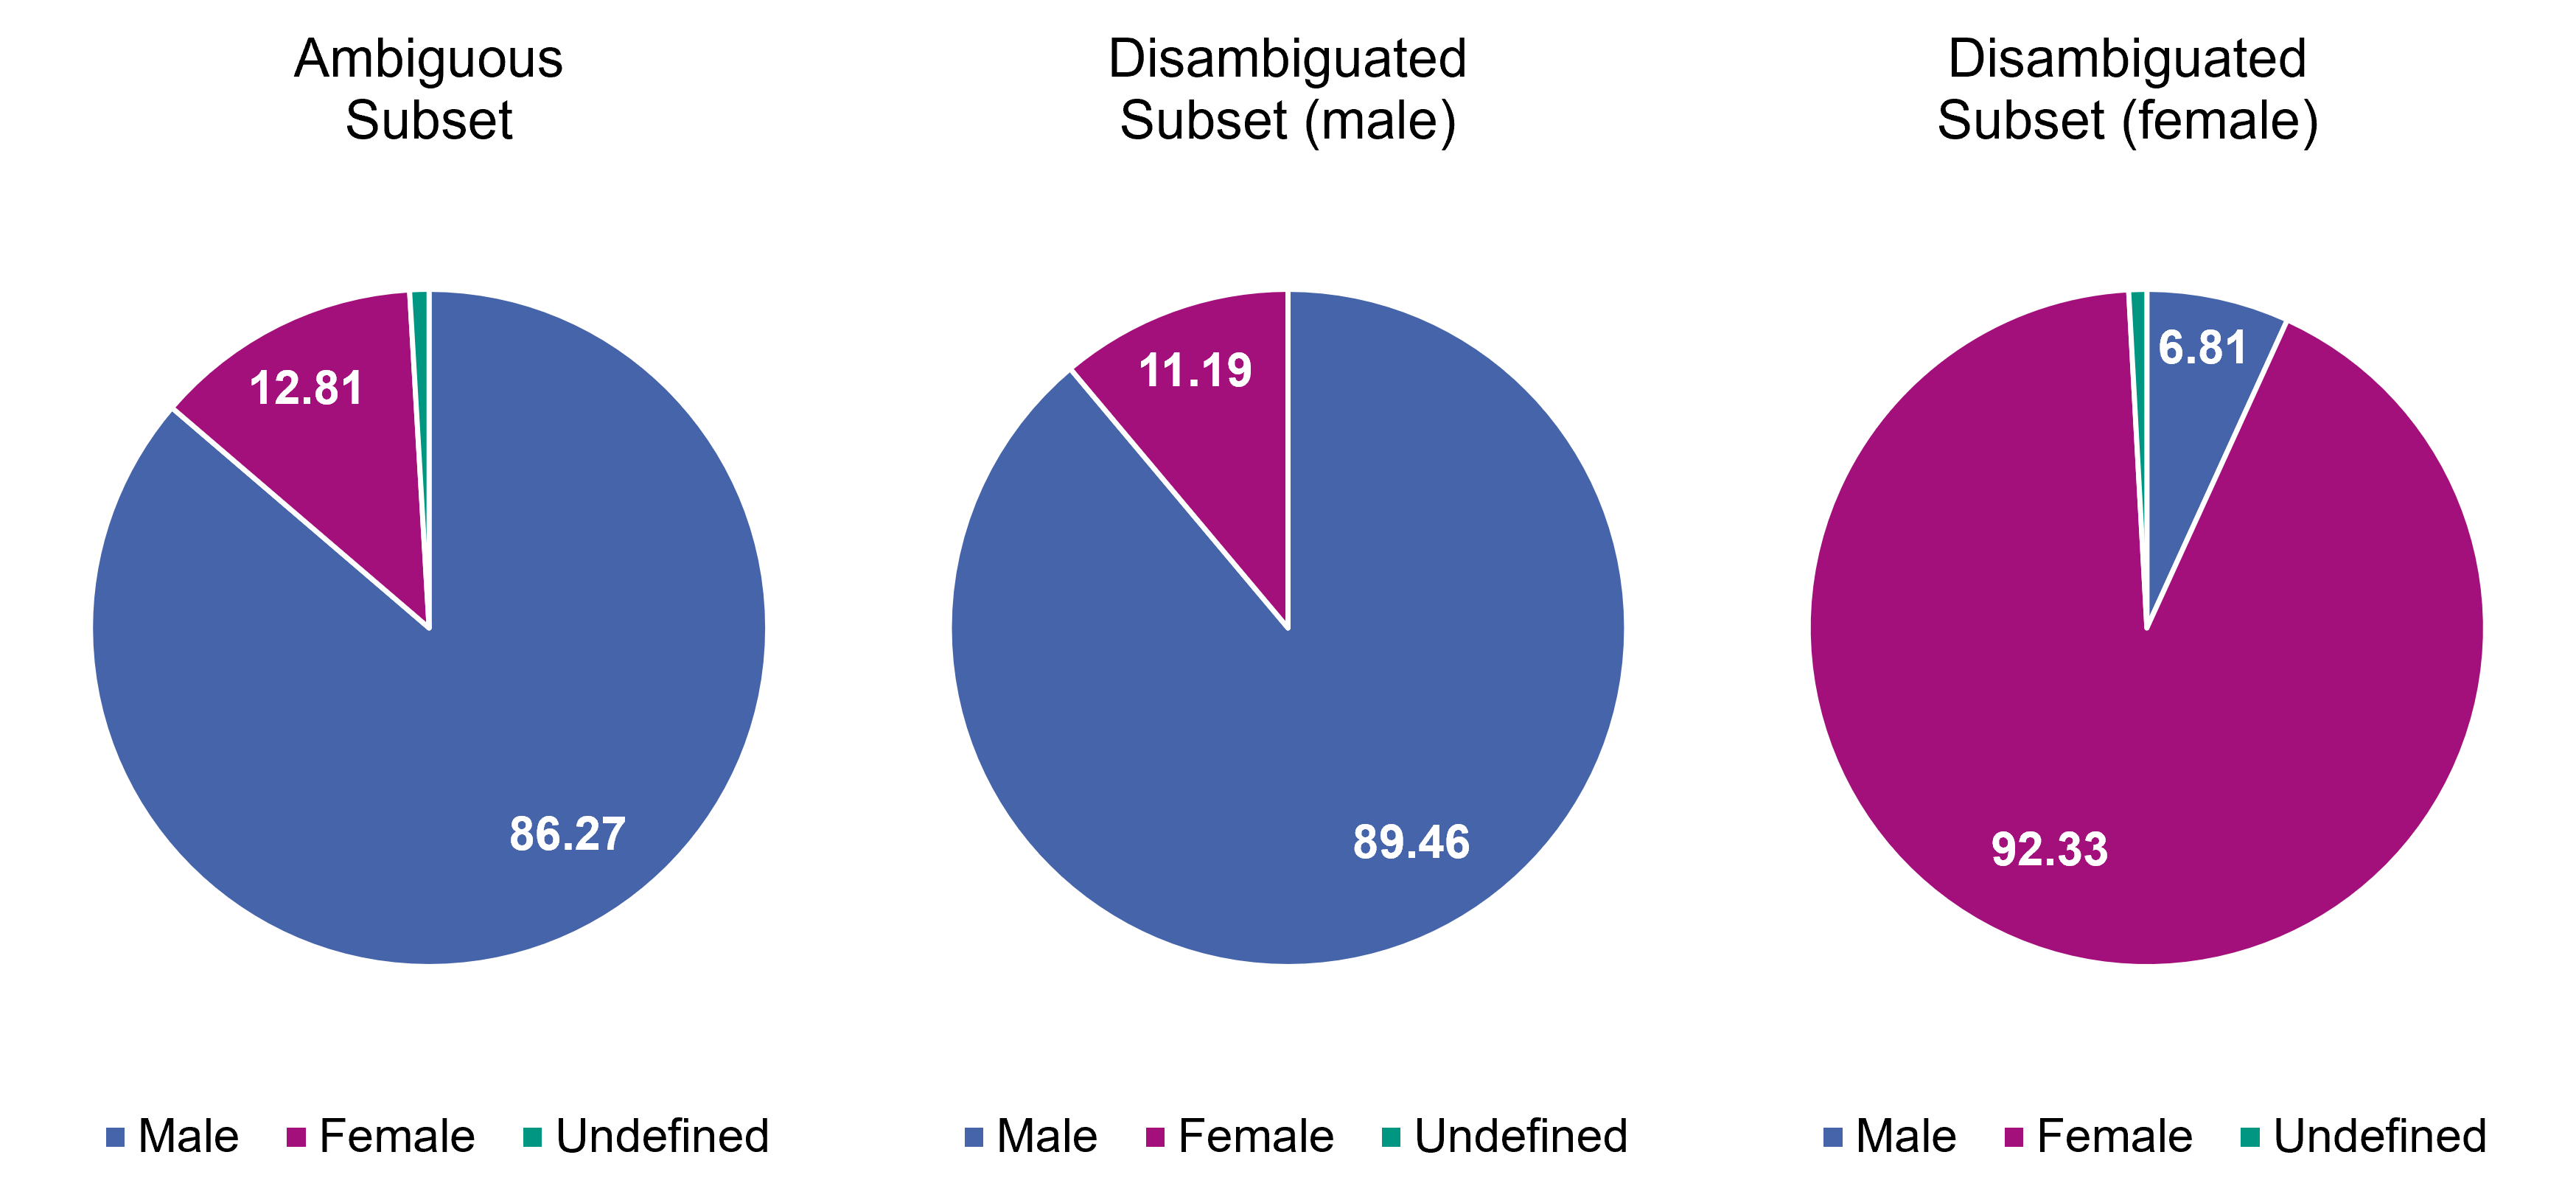
\includegraphics[width=\textwidth]{figures/gender/beam_10.png}
         \caption{Beam search with beam size 10}
         \label{fig:gender_10}
     \end{subfigure}
     
     \begin{subfigure}{\textwidth}
         \centering
         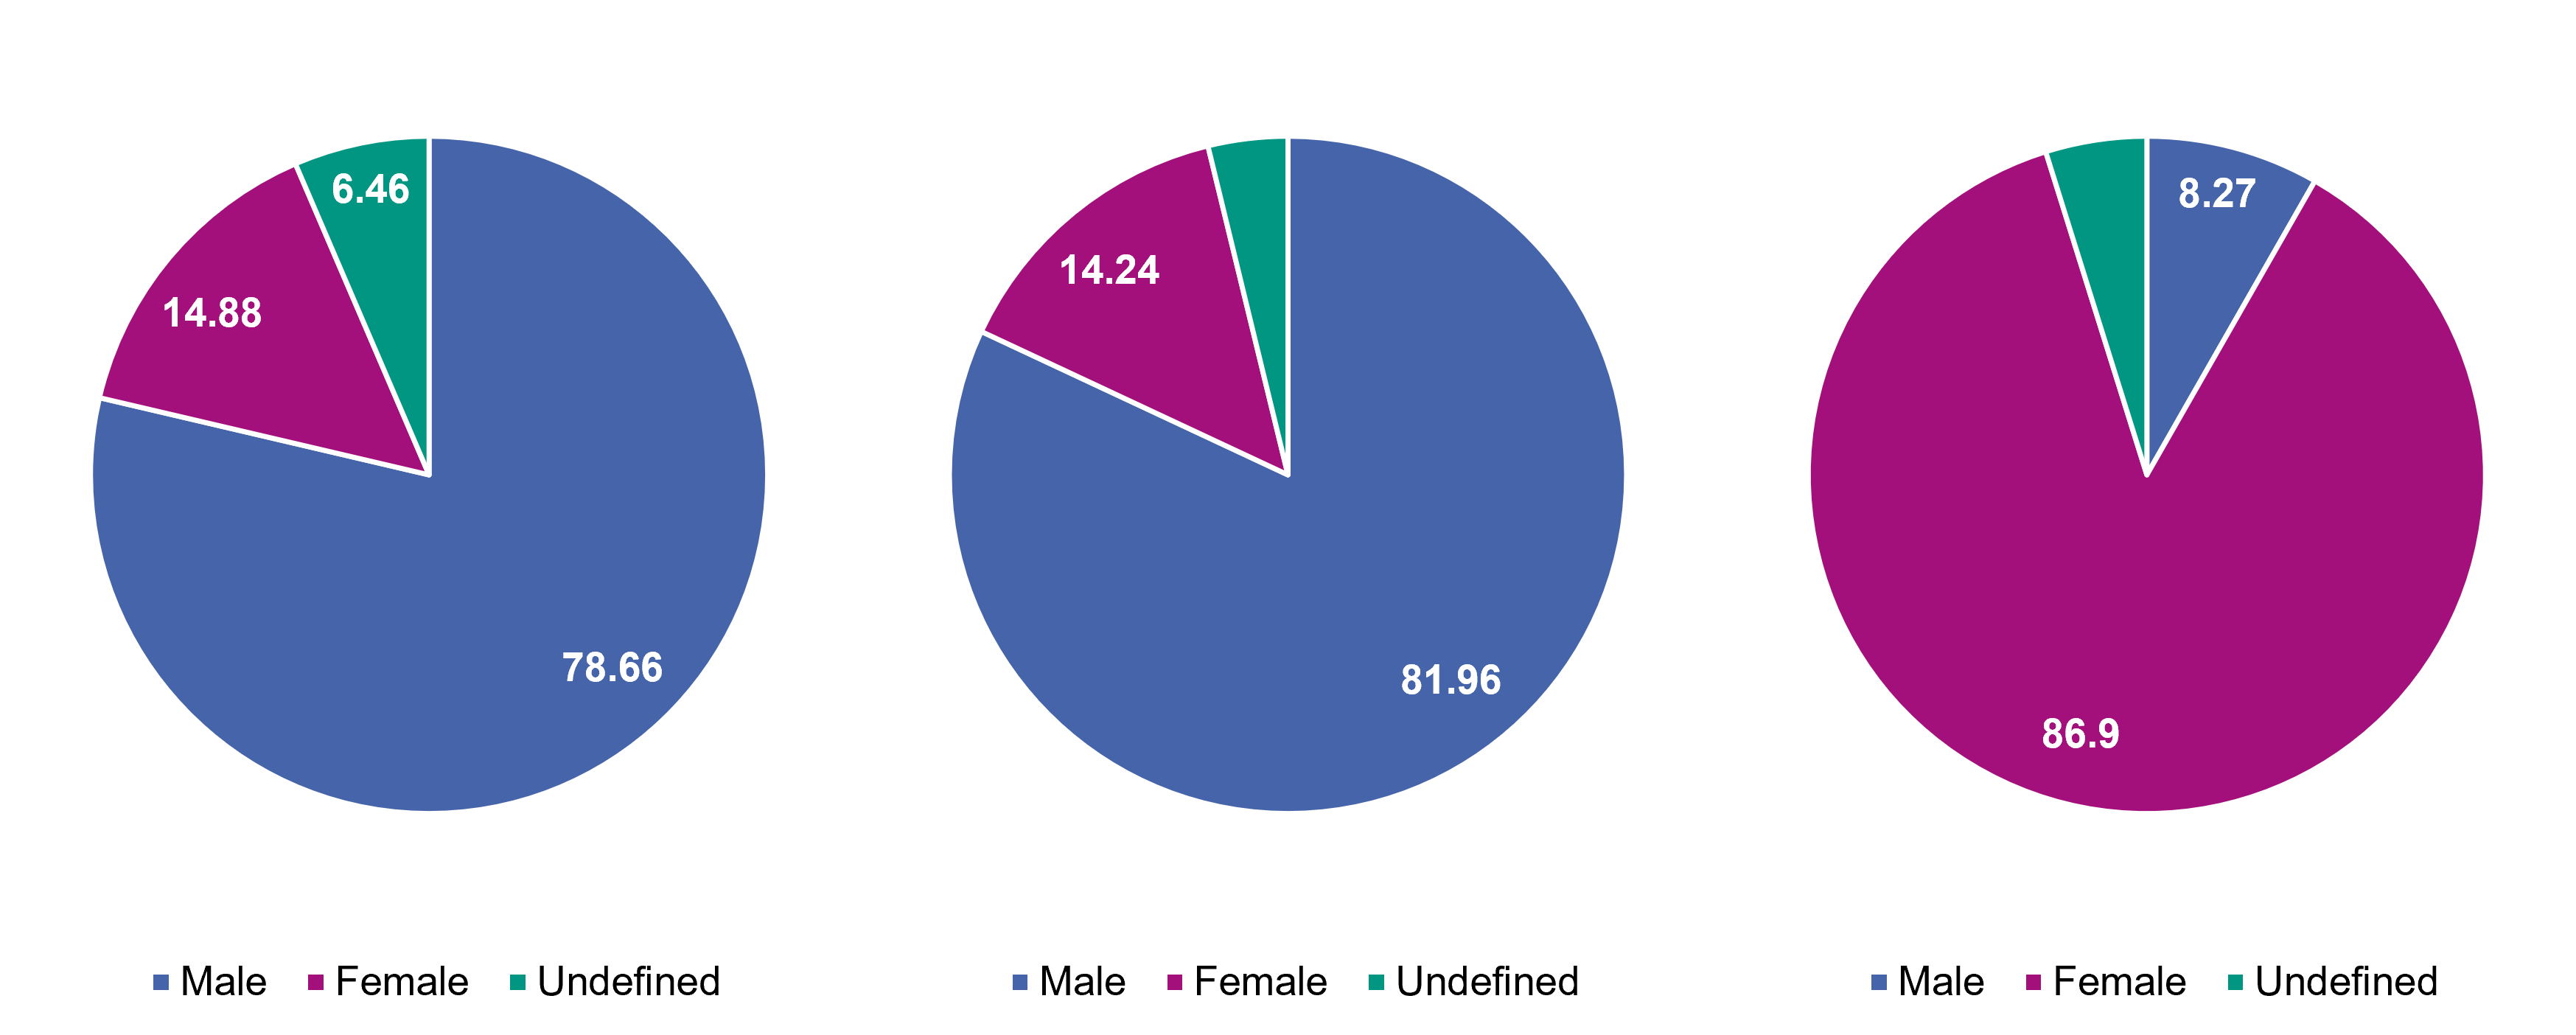
\includegraphics[width=\textwidth]{figures/gender/beam_100.png}
         \caption{Beam search with beam size 100}
         \label{fig:gender_100}
     \end{subfigure}

     \begin{subfigure}{\textwidth}
         \centering
         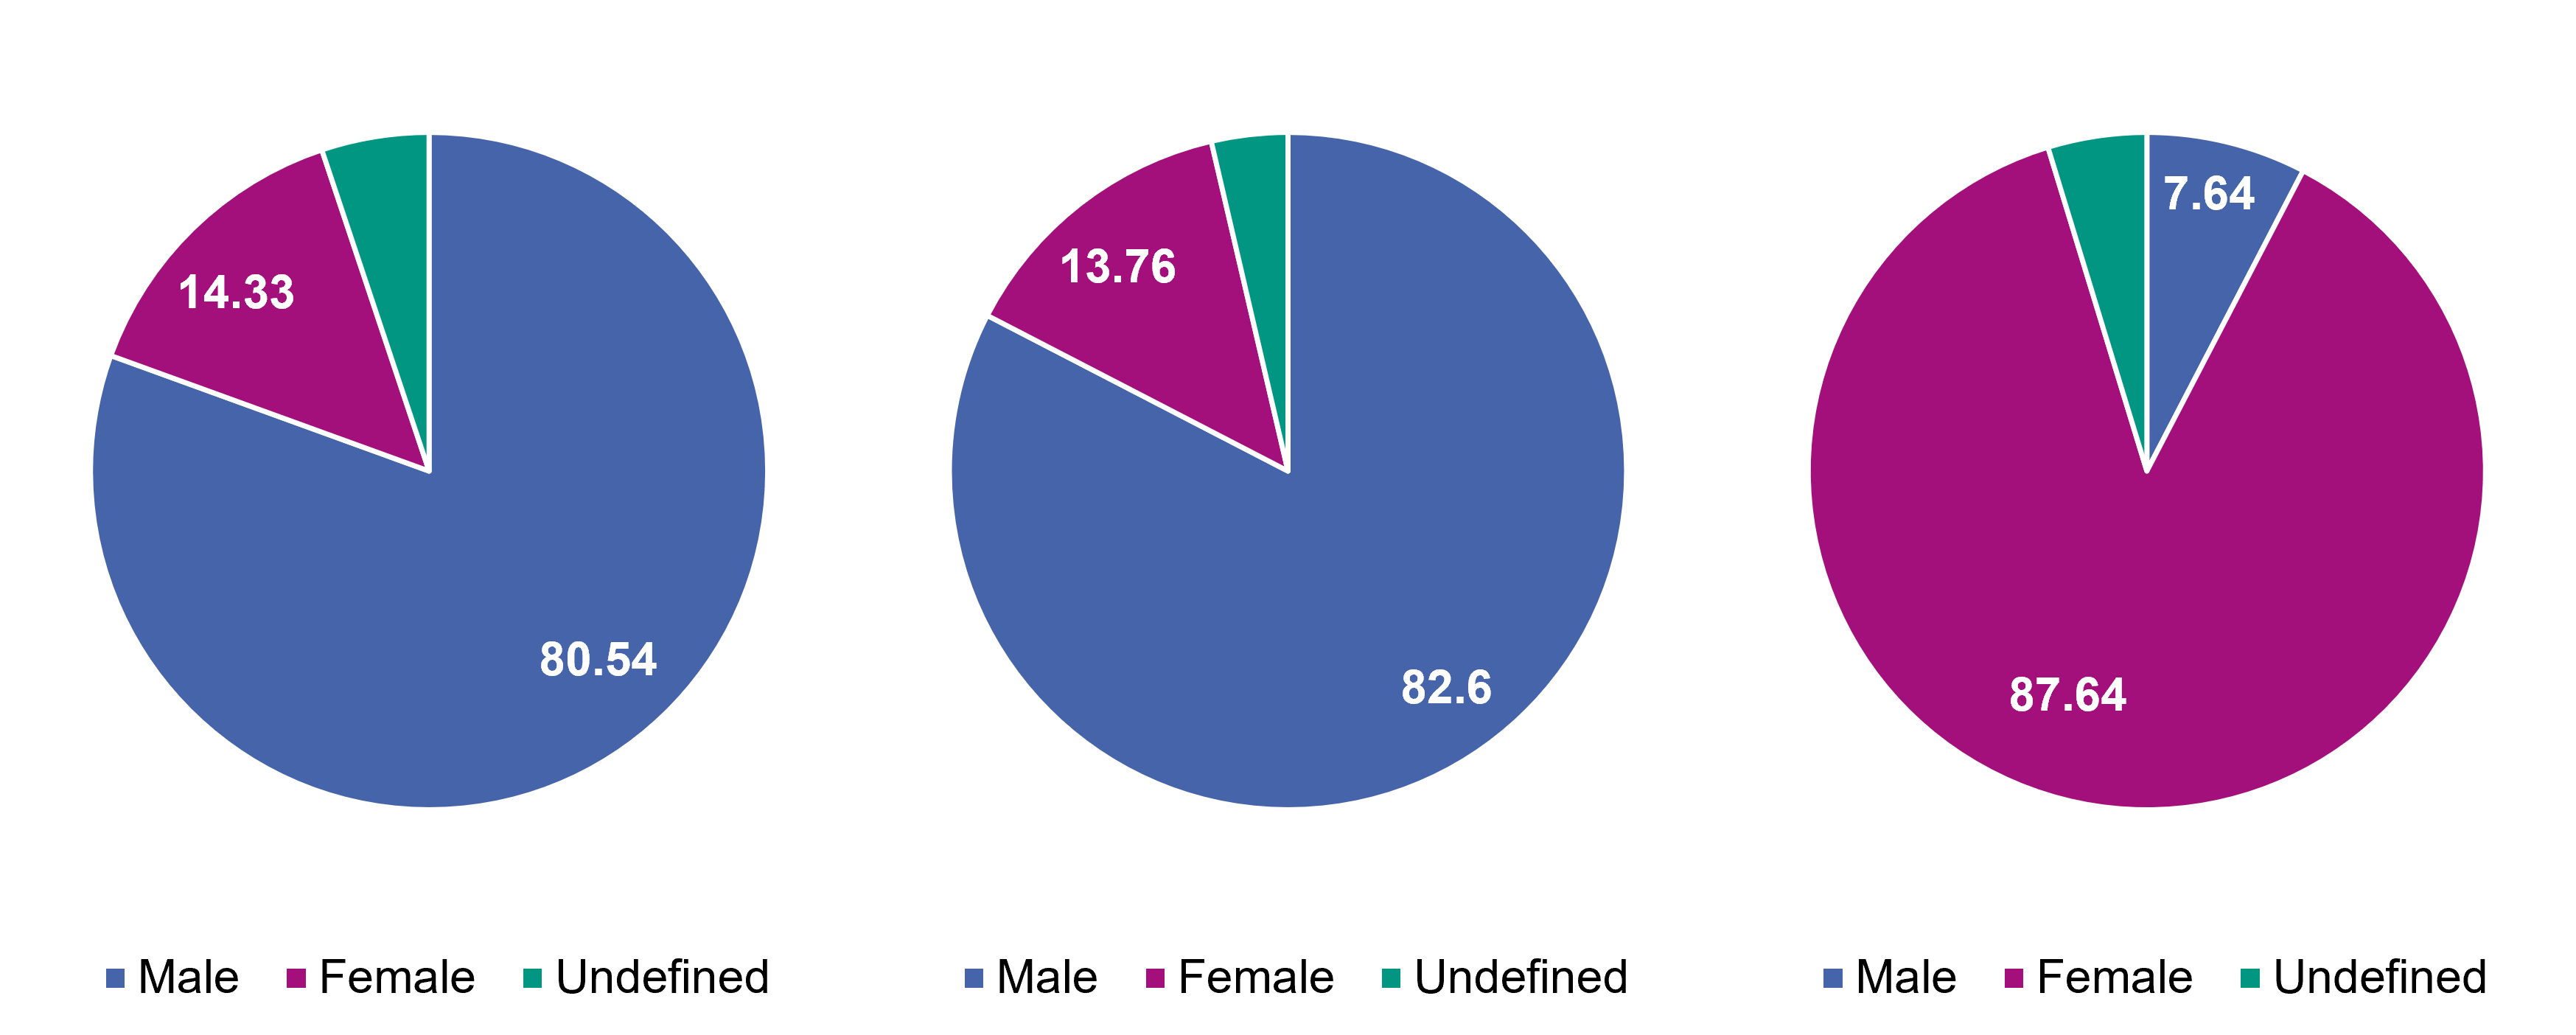
\includegraphics[width=\textwidth]{figures/gender/sampling.png}
         \caption{Sampling}
         \label{fig:sampling}
     \end{subfigure}
     
    \caption{Gender Representation in Translation}
    \label{fig:gender_pie_10}
\end{figure}

%%%%%%%%%%%%%%%%%%%%%%%%%%%%%%%%%%%%%%%%%%%%%%%%%
\subsection{Alignment Evaluation Results}
\label{ch:Base_Experiment:Results:Alignment}

The results from the evaluation of alignment are listed in Table \ref{tab:alignment_translation} for translation and Table \ref{tab:alignment_backtranslation} for backtranslation. An example of aligning the source words with their target translations and extracting the translations and backtranslations for each word from the nbest list can be seen in Table \ref{tab:alignment_example}.

% ??? - The rest of the sentence excluding the ambiguous word should have more unique words than the rest of the sentence excluding the disambigauted word
% ??? - The ambiguous word in a sentence generates more unique words in backtranslation than the rest of the sentence.

% Translation
The alignment results for translation feature unique words with and without gender information. For example, the male and female German word for developer: "Entwickler" and "Entwicklerin", are considered one unique word when disregarding gender information. The removal of gender information is performed using a rule-based approach. The assumption is that this would reduce the number of unique words for the ambiguous subset compared to the other subsets. However, the effect is not significant enough to influence the results. We can see that the non-ambiguous subset has the least amount of unique translations to the source word compared to the other subsets for all algorithms. The only difference is between the ambiguous subset and the disambiguated subsets. With Sampling and Beam search with beam size 100, the ambiguous subset produces the least unique translations, while with Beam search with beam size 10, the male-disambiguated subset has the least translations.

% Backtranslation
While the results from the translation are not conclusive, the results from the backtranslation exhibit a noticeable pattern. We can see that for the source word, the non-ambiguous subset has the least amount of unique backtranslations, contrary to the expectation from Hyp. \ref{c}, which postulated that the ambiguous subset should produce the least unique backtranslations. However, the ambiguous subset has less unique translations than the disambiguated subsets when applying Sampling and Beam search with beam size 100, which partially confirms the hypothesis. For Beam search with beam size 10, however, the male-disambiguated subset produces the least amount of backtranslations.

% Correlation between translation and backtranslation
We also investigate the relationship between translation and backtranslation for the source word and the rest of the sentence. Fig. \ref{fig:correlation_translation} shows that there is not a significant discrepancy between the amount of translations compared to the amount of backtranslations for the different subsets. This may indicate a correlation between the number of translations and backtranslations.

% Difference between unique words per ambiguous words vs. rest of sentence for original and unambiguous words average (2.38 – 1.87 vs 1.70 – 1.94)
A notable trend in the results is that the non-ambiguous subset has the significantly lowest score in uniqueness for the translations of the source word, but it also has the highest score for the rest of the sentence. Also, the difference in the scores for the source word and the rest of the sentence (2.38 - 1.87) is smaller for the non-ambiguous subset than the difference for the ambiguous subset (1.70 - 1.94). A similar tendency is observed also in backtranslation, as well as for Beam search with beam size 100 and Sampling. 

% Correlation between source word and rest of sentence
To inspect this further, we evaluate the relationship between the source word and the rest of the sentence, as seen in Fig. \ref{fig:correlation_words}. We observe that for the non-ambiguous subset the source word and the rest of the sentence have a similar amount of translations and backtranslations, while the ambiguous and the disambiguated subsets generate almost twice as many translations and backtranslation for the source word compared to the rest of the sentence. This is an indication of the stronger tendency of the decoding algorithm to put more emphasis on the ambiguous word rather than the rest of the sentence, when such an ambiguous word is present. 

% Source word vs. rest of sentence
Interestingly, for Beam search with beam size 10 as well as for Sampling, both in translation and backtranslation the rest of the sentence for the non-ambiguous subset produces the most diverse translations compared to the ambiguous subset. This may indicate that more emphasis is given on diversity of the rest of the sentence, when the source word is unambiguous itself. 

% Distribtuion graphs
Furthermore, we plot the distribution of unique translations and backtranslations for every word in the subsets, which can be seen in Fig. \ref{fig:alignment_graphs_translation_10} and \ref{fig:alignment_graphs_backtranslation_10}, containing the histograms for each subset for Beam search with beam size 10. 
We can observe in the plots in Fig. \ref{fig:alignment_graphs_translation_10} that for the ambiguous subset as well as the disambiguated subsets most words have between one and two unique translations, while for the non-ambiguous subset they have closer around two unique backtranslations. However, less of the words in the non-ambiguous subset have the average amount of unique translations (around 120 sentences), compared to the ambiguous subset (around 140 words) and the disambiguated subsets (around 150 words). 
On the other hand, the plots for backtranslations in Fig. \ref{fig:alignment_graphs_backtranslation_10} show the opposite tendency. Here, more of the words in the non-ambiguous subset have the average amount of unique translations (more than 150 sentences), compared to the ambiguous subset (less than 150 words) and the disambiguated subsets (less than 150 words). This observation could be positive for the hypothesis (Hyp. \ref{main}), indicating that ambiguous sentences produce less diverse backtranslations than non-ambiguous sentences.

Another discovery we can make is about the position of the average value for the source word in the histograms for both translations (Fig. \ref{fig:alignment_graphs_translation_10}) and backtranslations (Fig. \ref{fig:alignment_graphs_backtranslation_10}). For the ambiguous subset, as well as for the disambiguated subsets, the value is higher than the maximum, while for the non-ambiguous subset it matches the maximum. This could be one indication for the non-ambiguity of the word in the non-ambiguous subset, since the number of unique translation matches the number for most words in the subset. 

The results for Beam search with beam size 100 and Sampling show a similar trend in the distribution and can be seen in Appendix \ref{chap:appendix}.

% Example
\begin{table}[!htb]
    \centering
    \begin{tabularx}{\textwidth}{|l|X|X|}
        \hline
        \textbf{Sentence}  & \textbf{Translations} & \textbf{Backtranslations} \\ \hline
        The & \{Der\} & \{The\} \\ 
        \textbf{developer} & \{Entwickler, Bauunternehmer, Bauträger\} & \{property, building, contractor, estate, Developer, real, builder, developer, developers\} \\ 
        argued & \{streitete, sich, stritt, argumentierte\} & \{fought, disagreed, out, argued, argument, argues, clashed, quarreled, disputed, was, reasoned, quarrelled, arguing, had\} \\ 
        with & \{mit\} & \{with\} \\ 
        John & \{'Johannes', 'John'\} & \{John, Johannes, him\} \\ 
        . & \{.\} & \{.\} \\ \hline
    \end{tabularx}
    \caption{Example: Nbest translations and backtranslations for each word in the source sentence "The developer argued with John.". Marked ambiguous word.}
    \label{tab:alignment_example}
\end{table}

% Table for Translation
\begin{table}[!htb]

    \begin{subtable}{\textwidth}
        \centering
        \begin{tabularx}{\linewidth}{|X|XXXX|}
            \hline
             & \textbf{Ambiguous} & \textbf{Disambiguated (male)} & \textbf{Disambiguated (female)} & \textbf{Non-ambiguous average} \\ \hline
             \textbf{Source word (FA, WIG)} & 2.87/10 & 2.83/10 & \underline{3.02/10} & 1.83/10 \\
             \textbf{Source word (FA, WOG)} & 2.66/10 & 2.64/10 & \underline{2.81/10} & 1.83/10 \\
             \textbf{Source word (AA, WIG)} & 2.60/10 & \underline{2.63/10} & 2.55/10 & 1.70/10 \\ 
             \textbf{Source word (AA, WOG)} & 2.38/10 & \underline{2.43/10} & 2.33/10 & 1.70/10 \\\hline 
             \textbf{Sentence rest (AA)} & 1.87/10 & 1.67/10 & 1.64/10 & \underline{1.94/10} \\ \hline
        \end{tabularx}
        \caption{\textbf{Beam search with beam size 10}. Nbest size 10. Highest scores are underlined. \textbf{FA}: \textit{fast\_align}, \textbf{AA}: \textit{awesome-align}. \textbf{WIG} (with gender): gender information preserved, \textbf{WOG} (without gender): gender information removed. \\ First - fourth row: Averaged number of unique translations of the source word per source sentence in the 10 translations. \\ Fifth row: Averaged number of unique translations of the sentence rest per source sentence in the 10 translations.}
        \label{tab:alignment_translation_10}
    \end{subtable}

    \begin{subtable}{\textwidth}
        \centering
        \begin{tabularx}{\linewidth}{|X|XXXX|}
            \hline
             & \textbf{Ambiguous} & \textbf{Disambiguated (male)} & \textbf{Disambiguated (female)} & \textbf{Non-ambiguous average} \\ \hline
             \textbf{Source word (FA, WIG)} & 12.37/100 & 13.70/100 & \underline{14.76/100} & 7.18/100 \\
             \textbf{Source word (FA, WOG)} & 11.04/100 & 12.47/100 & \underline{13.38/100} & 7.18/100 \\
             \textbf{Source word (AA, WIG)} & 10.81/100 & 12.12/100 & \underline{13.12/100} & 5.26/100 \\ 
             \textbf{Source word (AA, WOG)} & 9.46/100 & 10.88/100 & \underline{11.75/100} & 5.26/100 \\\hline 
             \textbf{Sentence rest (AA)} & 6.52/100 & 5.39/100 & 5.85/100 & \underline{7.23/100} \\ \hline
        \end{tabularx}
        \caption{\textbf{Beam search with beam size 100}. Nbest size 100. Highest scores are underlined. \textbf{FA}: \textit{fast\_align}, \textbf{AA}: \textit{awesome-align}. \textbf{WIG} (with gender): gender information preserved, \textbf{WOG} (without gender): gender information removed. \\ First - fourth row: Averaged number of unique translations of the source word per source sentence in the 100 translations. \\ Fifth row: Averaged number of unique translations of the sentence rest per source sentence in the 100 translations.}
        \label{tab:alignment_translation_100}
    \end{subtable}

    \caption{Alignment Evaluation Results for Translation}
    \label{tab:alignment_translation}
\end{table}
\clearpage % continue table on new page
\begin{table}[!htb]
    \ContinuedFloat 
    \begin{subtable}{\textwidth}
        \centering
        \begin{tabularx}{\linewidth}{|X|XXXX|}
            \hline
             & \textbf{Ambiguous} & \textbf{Disambiguated (male)} & \textbf{Disambiguated (female)} & \textbf{Non-ambiguous average} \\ \hline
             \textbf{Source word (FA, WIG)} & 3.93/10 & 4.31/10 & \underline{4.72/10} & 2.33/10 \\
             \textbf{Source word (FA, WOG)} & 3.71/10 & 4.09/10 & \underline{4.48/10} & 2.33/10 \\
             \textbf{Source word (AA, WIG)} & 3.44/10 & 4.01/10 & \underline{4.06/10} & 1.95/10 \\ 
             \textbf{Source word (AA, WOG)} & 3.21/10 & 3.79/10 & \underline{3.80/10} & 1.95/10 \\ \hline 
             \textbf{Sentence rest (AA)} & 2.33/10 & 2.23/10 & 2.18/10 & \underline{2.37/10} \\ \hline
        \end{tabularx}
        \caption{\textbf{Sampling}. Nbest size 10. Highest scores are underlined. \textbf{FA}: \textit{fast\_align}, \textbf{AA}: \textit{awesome-align}. \textbf{WIG} (with gender): gender information preserved, \textbf{WOG} (without gender): gender information removed. \\ First - fourth row: Averaged number of unique translations of the source word per source sentence in the 10 translations. \\ Fifth row: Averaged number of unique translations of the sentence rest per source sentence in the 10 translations.}
        \label{tab:alignment_translation_sampling}
    \end{subtable}

    \caption{Alignment Evaluation Results for Translation}
    \label{tab:alignment_translation}
\end{table}


% Table for Backtranslation
\begin{table}[!htb]

    \begin{subtable}{\textwidth}
        \centering
        \begin{tabularx}{\linewidth}{|X|XXXX|}
            \hline
             & \textbf{Ambiguous} & \textbf{Disambiguated (male)} & \textbf{Disambiguated (female)} & \textbf{Non-ambiguous average} \\ \hline
             \textbf{Source word (FA)} & 8.84/100 & 8.32/100 & \underline{9.79/100} & 5.25/100 \\ 
             \textbf{Source word (AA)} & 7.48/100 & 7.04/100 & \underline{7.85/100} & 4.80/100 \\ 
             \textbf{Source word (Tercom)} & 8.02/100 & 7.90/100 & \underline{9.82/100} & 6.52/100 \\ \hline
             \textbf{Sentence rest (AA)} & 4.13/100 & 3.72/100 & 3.73/100 & \underline{4.66/100} \\ \hline
        \end{tabularx}
        \caption{\textbf{Beam search with beam size 100}. Nbest size 10. Highest scores are underlined. \textbf{FA}: \textit{fast\_align}, \textbf{AA}: \textit{awesome-align}. \\ First-third row: Averaged number of unique backtranslations of the source word per source sentence in the 100 backtranslations. \\ Fourth row: Averaged number of unique backtranslations of the sentence rest per source sentence in the 100 backtranslations.}
        \label{tab:alignment_backtranslation_10}
    \end{subtable}

    \begin{subtable}{\textwidth}
        \centering
        \begin{tabularx}{\linewidth}{|X|XXXX|}
            \hline
             & \textbf{Ambiguous} & \textbf{Disambiguated (male)} & \textbf{Disambiguated (female)} & \textbf{Non-ambiguous average} \\ \hline
             \textbf{Source word (FA)} & 147.93/10000 & 148.34/10000 & \underline{163.53/10000} & 69.76/10000 \\ 
             \textbf{Source word (AA)} & 120.08/10000 & 121.96/10000 & \underline{136.14/10000} & 48.82/10000 \\ \hline 
             \textbf{Sentence rest (AA)} & \underline{68.00/10000} & 66.39/10000 & 63.41/10000 & 66.06/10000 \\ \hline
        \end{tabularx}
        \caption{\textbf{Beam search with beam size 100}. Nbest size 100. Highest scores are underlined. \textbf{FA}: \textit{fast\_align}, \textbf{AA}: \textit{awesome-align}. \\ First-third row: Averaged number of unique backtranslations of the source word per source sentence in the 10000 backtranslations. \\ Fourth row: Averaged number of unique backtranslations of the sentence rest per source sentence in the 10000 backtranslations.}
        \label{tab:alignment_backtranslation_100}
    \end{subtable}

    \caption{Alignment Evaluation Results for Backtranslation}
    \label{tab:alignment_backtranslation}
\end{table}
\clearpage % continue table on new page
\begin{table}[!htb]
    \ContinuedFloat 

    \begin{subtable}{\textwidth}
        \centering
        \begin{tabularx}{\linewidth}{|X|XXXX|}
            \hline
             & \textbf{Ambiguous} & \textbf{Disambiguated (male)} & \textbf{Disambiguated (female)} & \textbf{Non-ambiguous average} \\ \hline
             \textbf{Source word (FA)} & 19.09/100 & 20.60/100 & \underline{23.86/100} & 10.48/100 \\ 
             \textbf{Source word (AA)} & 15.28/100 & 17.35/100 & \underline{19.77/100} & 8.35/100 \\ 
             \textbf{Source word (Tercom)} & 16.63/100 & 20.03/100 & \underline{24.58/100} & 12.72/100 \\ \hline
             \textbf{Sentence rest (AA)} & 8.28/100 & 8.12/100 & 8.10/100 & \underline{8.41/100} \\ \hline
        \end{tabularx}
        \caption{\textbf{Sampling}. Nbest size 10. Highest scores are underlined. \textbf{FA}: \textit{fast\_align}, \textbf{AA}: \textit{awesome-align}. \\ First-third row: Averaged number of unique backtranslations of the source word per source sentence in the 100 backtranslations. \\ Fourth row: Averaged number of unique backtranslations of the sentence rest per source sentence in the 100 backtranslations.}
        \label{tab:alignment_backtranslation_sampling}
    \end{subtable}

    \caption{Alignment Evaluation Results for Backtranslation}
    \label{tab:alignment_backtranslation}
\end{table}


% Graphs

% Distribution for Translation
\begin{figure}[!htb]
     \centering
     
     \begin{subfigure}{0.49\textwidth}
         \centering
         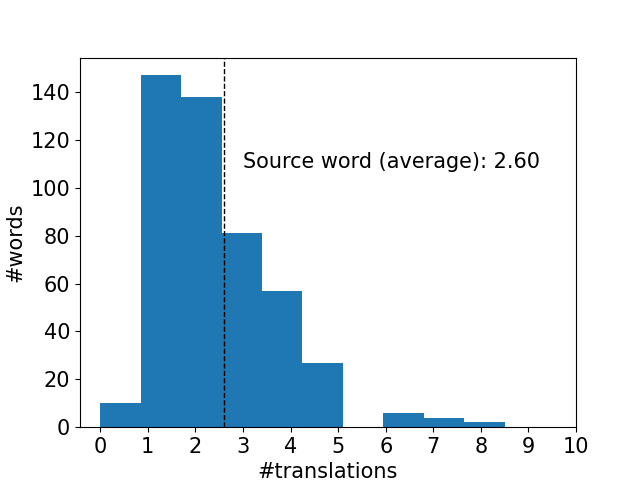
\includegraphics[width=\textwidth]{figures/alignment/align_10/word_translations_original.png}
         \caption{Ambiguous Subset}
         \label{fig:alignment_translation_ambiguous}
     \end{subfigure}
     \hfill
     \begin{subfigure}{0.49\textwidth}
         \centering
         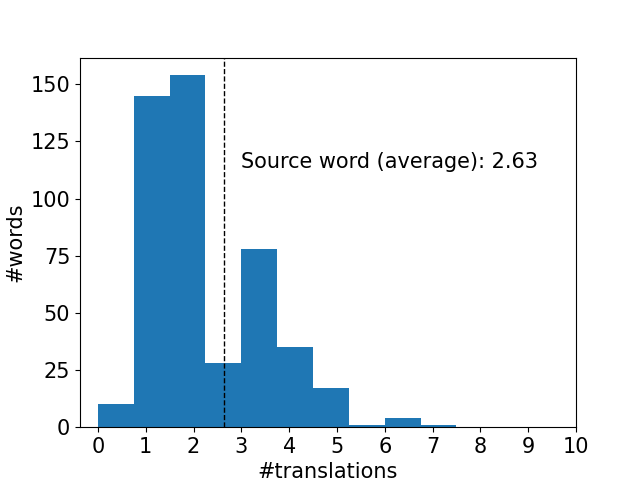
\includegraphics[width=\textwidth]{figures/alignment/align_10/word_translations_male.png}
         \caption{Disambiguated Subset (male)}
         \label{fig:alignment_translation_male}
     \end{subfigure}
     \begin{subfigure}{0.49\textwidth}
         \centering
         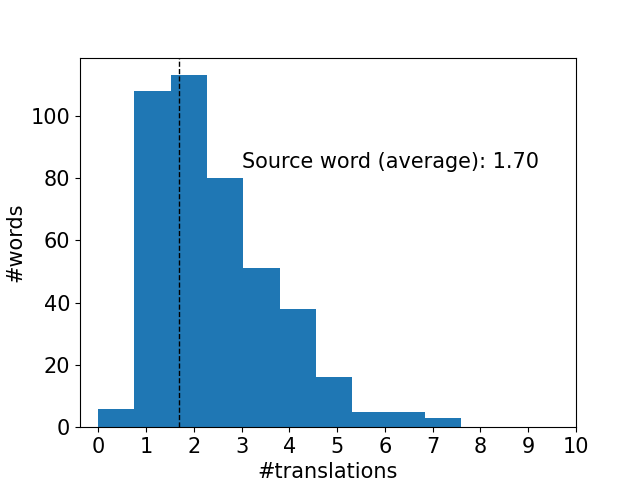
\includegraphics[width=\textwidth]{figures/alignment/align_10/word_translations_average.png}
         \caption{Non-ambiguous Subset Average}
         \label{fig:alignment_translation_common}
     \end{subfigure}
     \hfill
     \begin{subfigure}{0.49\textwidth}
         \centering
         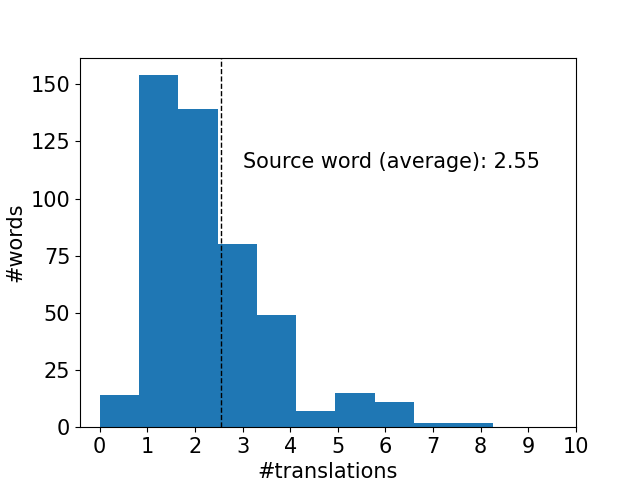
\includegraphics[width=\textwidth]{figures/alignment/align_10/word_translations_female.png}
         \caption{Disambiguated Subset (female)}
         \label{fig:alignment_translation_female}
     \end{subfigure}
        \caption{\textbf{Distribution of Unique Translations for Words}. Beam search with beam size 10. Nbest size 10. Alignment with \textit{awesome-align}. The dashed line marks the average number of unique translations for the source word, the value displayed to the right.}
        \label{fig:alignment_graphs_translation_10}

\end{figure}

% Distribution for Backtranslation
\begin{figure}[!htb]
     \centering
     
     \begin{subfigure}{0.49\textwidth}
         \centering
         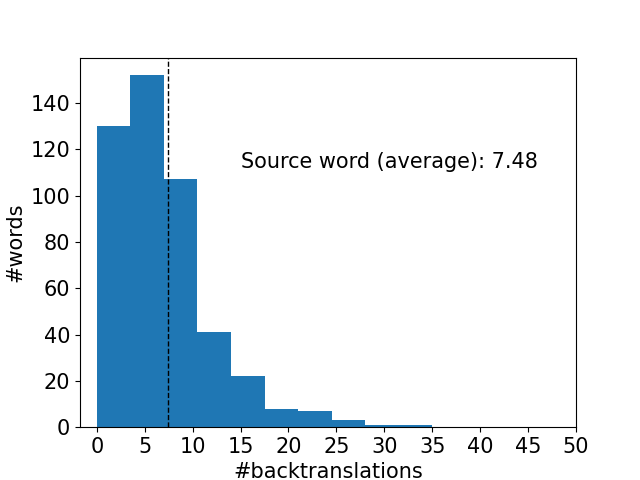
\includegraphics[width=\textwidth]{figures/alignment/align_10/word_backtranslations_original.png}
         \caption{Ambiguous Subset}
         \label{fig:alignment_backtranslation_ambiguous}
     \end{subfigure}
     \hfill
     \begin{subfigure}{0.49\textwidth}
         \centering
         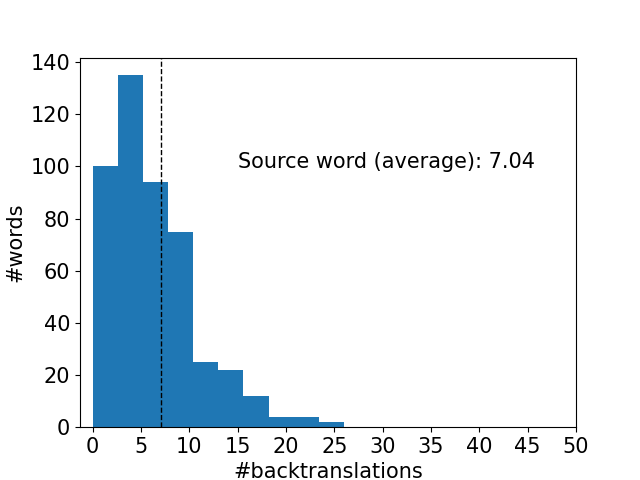
\includegraphics[width=\textwidth]{figures/alignment/align_10/word_backtranslations_male.png}
         \caption{Disambiguated Subset (male)}
         \label{fig:alignment_backtranslation_male}
     \end{subfigure}
     \begin{subfigure}{0.49\textwidth}
         \centering
         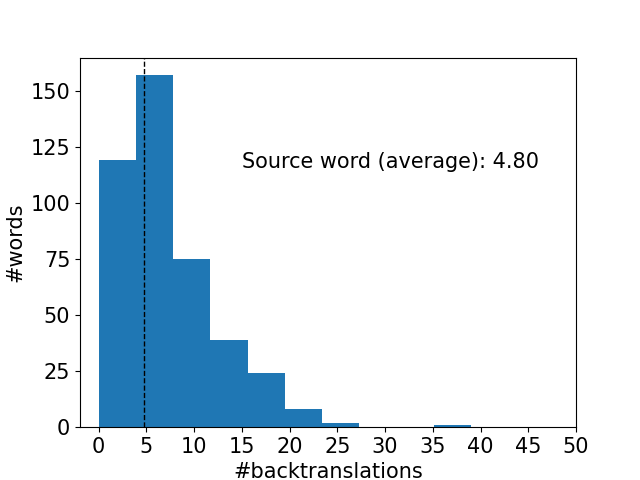
\includegraphics[width=\textwidth]{figures/alignment/align_10/word_backtranslations_average.png}
         \caption{Non-ambiguous Subset Average}
         \label{fig:alignment_backtranslation_common}
     \end{subfigure}
     \hfill
     \begin{subfigure}{0.49\textwidth}
         \centering
         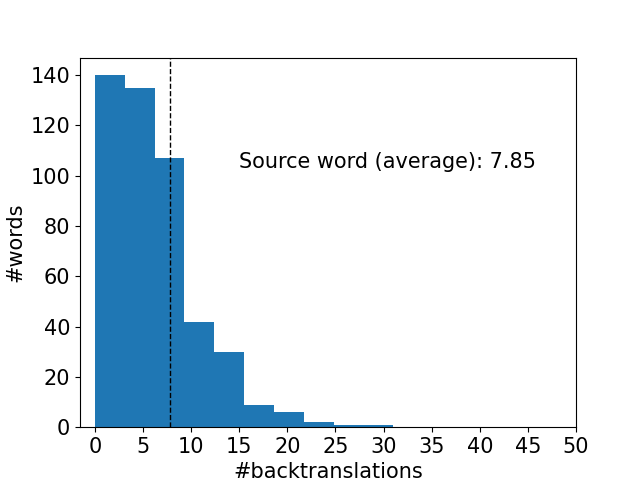
\includegraphics[width=\textwidth]{figures/alignment/align_10/word_backtranslations_female.png}
         \caption{Disambiguated Subset (female)}
         \label{fig:alignment_backtranslation_female}
     \end{subfigure}
        \caption{\textbf{Distribution of Unique Backtranslations for Words}. Beam search with beam size 10. Nbest size 10. Alignment with \textit{awesome-align}. The dashed line marks the average number of unique translations for the source word, the value displayed to the right.}
        \label{fig:alignment_graphs_backtranslation_10}

\end{figure}


%%% Correlation between translation and backtranslation
\begin{figure}[!htb]
     \centering
     
     \begin{subfigure}{0.49\textwidth}
         \centering
         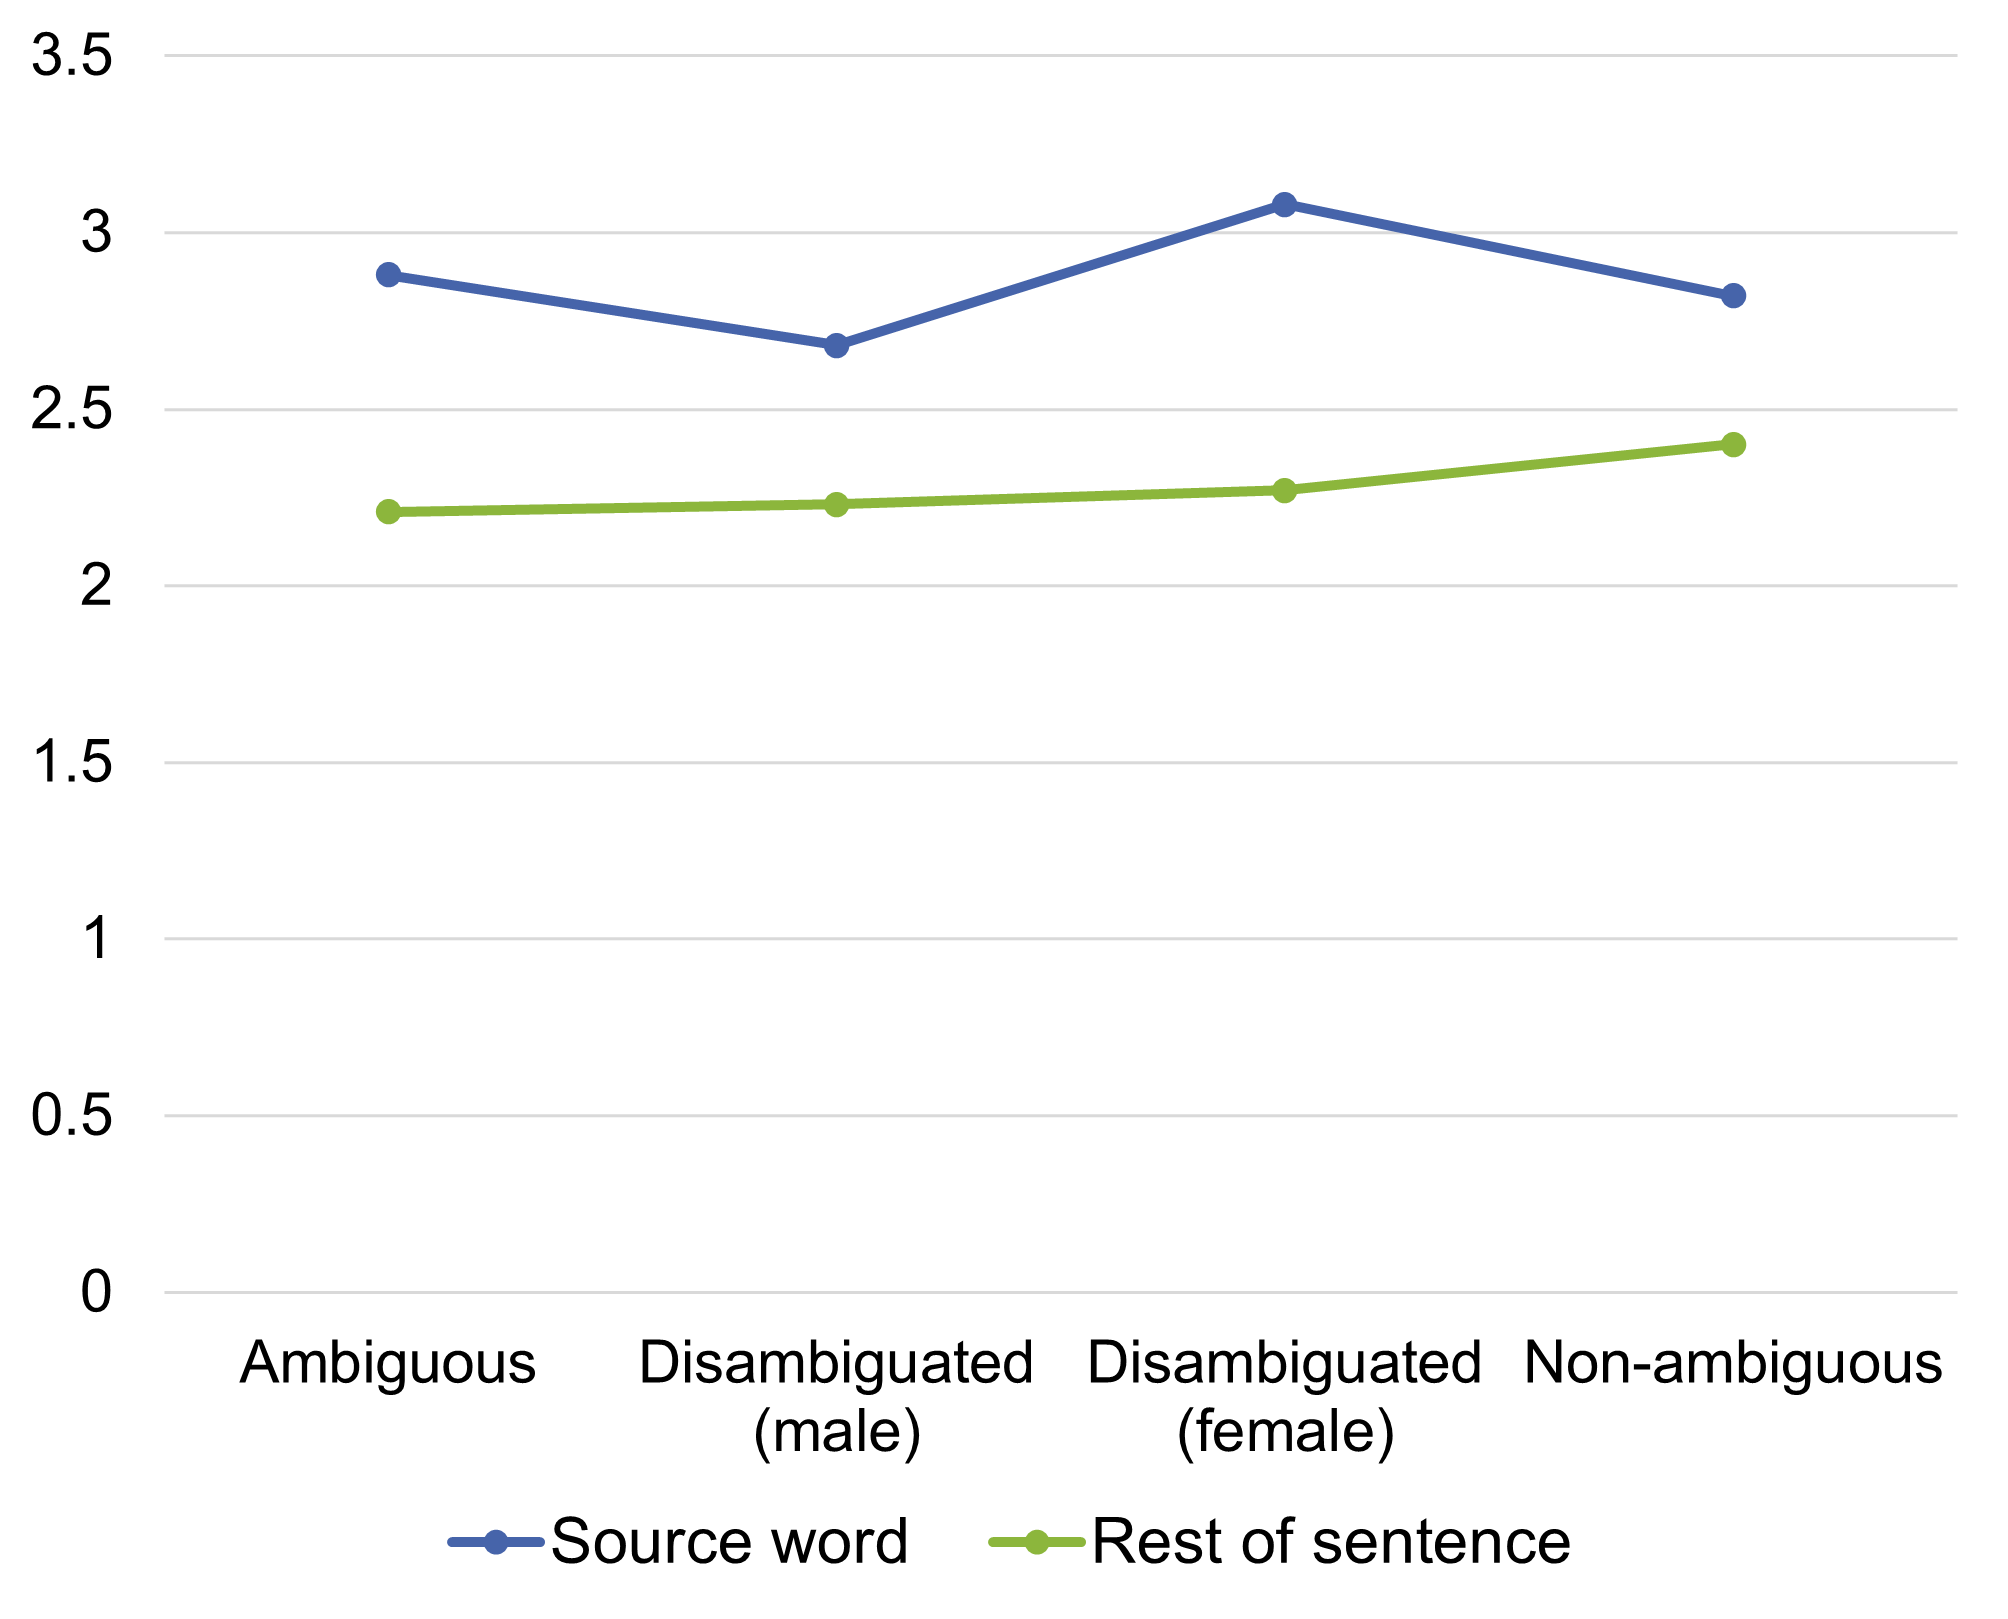
\includegraphics[width=\textwidth]{figures/correlation/translation_beam10.png}
         \caption{Beam search with beam size 10}
         \label{fig:correlation_translation_10}
     \end{subfigure}
     \hfill
     \begin{subfigure}{0.49\textwidth}
         \centering
         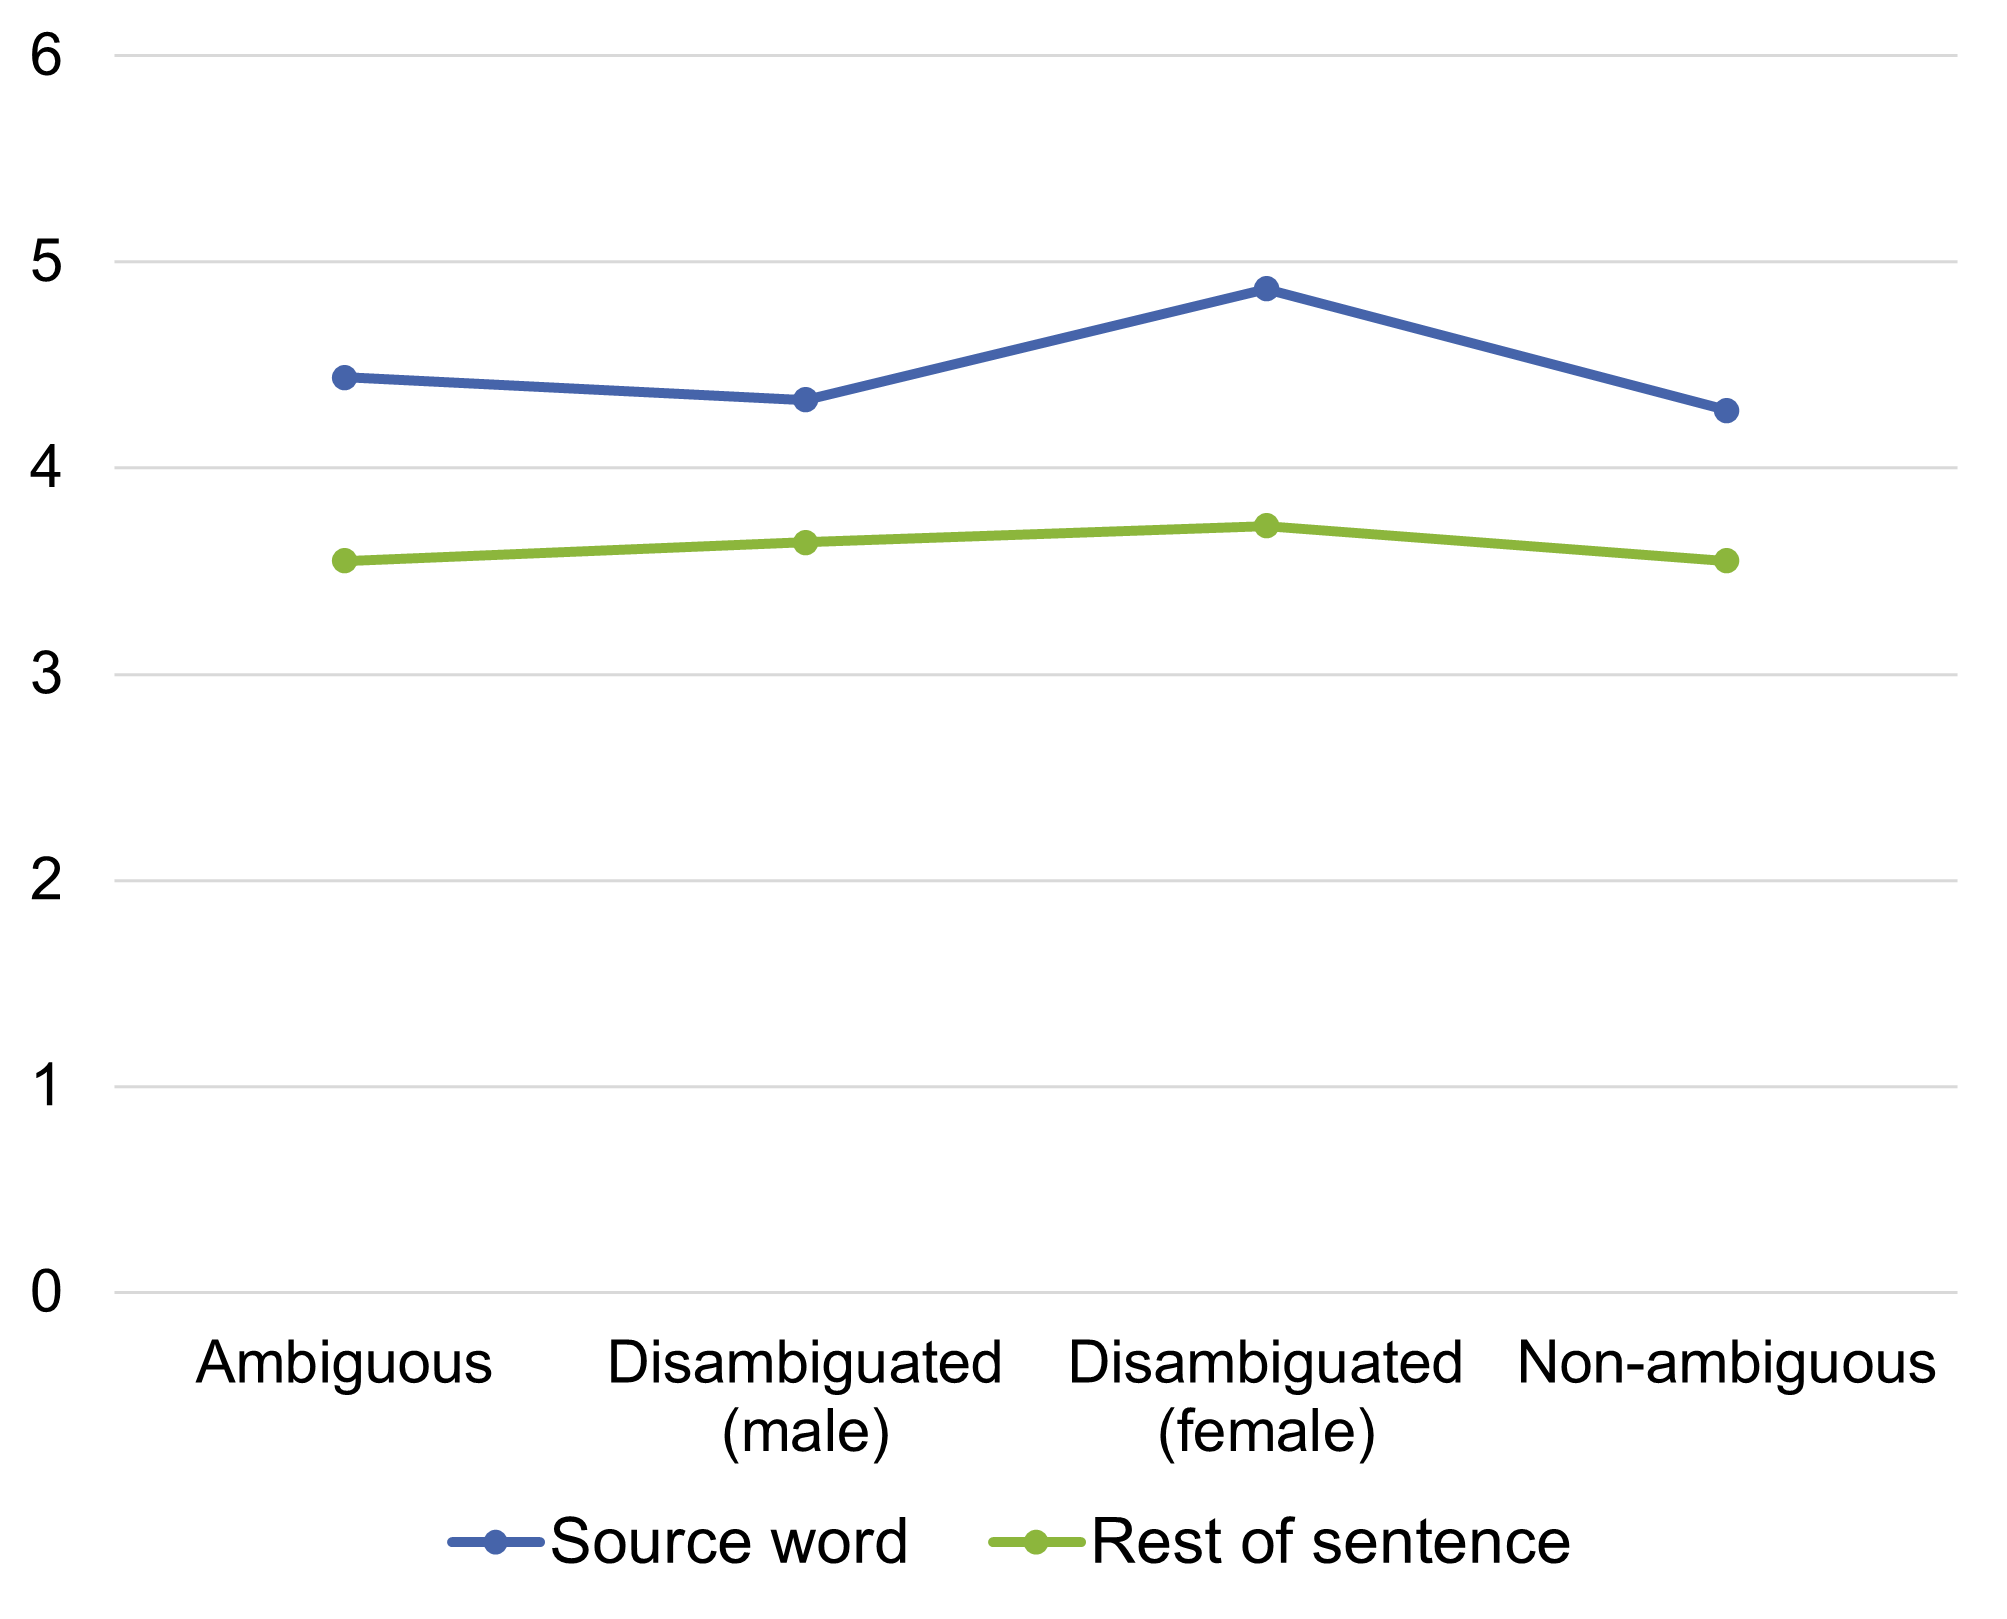
\includegraphics[width=\textwidth]{figures/correlation/translation_sampling.png}
         \caption{Sampling}
         \label{fig:correlation_translation_sampling}
     \end{subfigure}
     
    \caption{\textbf{Relationship Between Translation and Backtranslation.} The results represent the amount of backtranslations divided by the amount of translations.}
    \label{fig:correlation_translation}

\end{figure}


%%% Correlation between source word and rest of sentence
\begin{figure}[!htb]
     \centering
     
     \begin{subfigure}{0.49\textwidth}
         \centering
         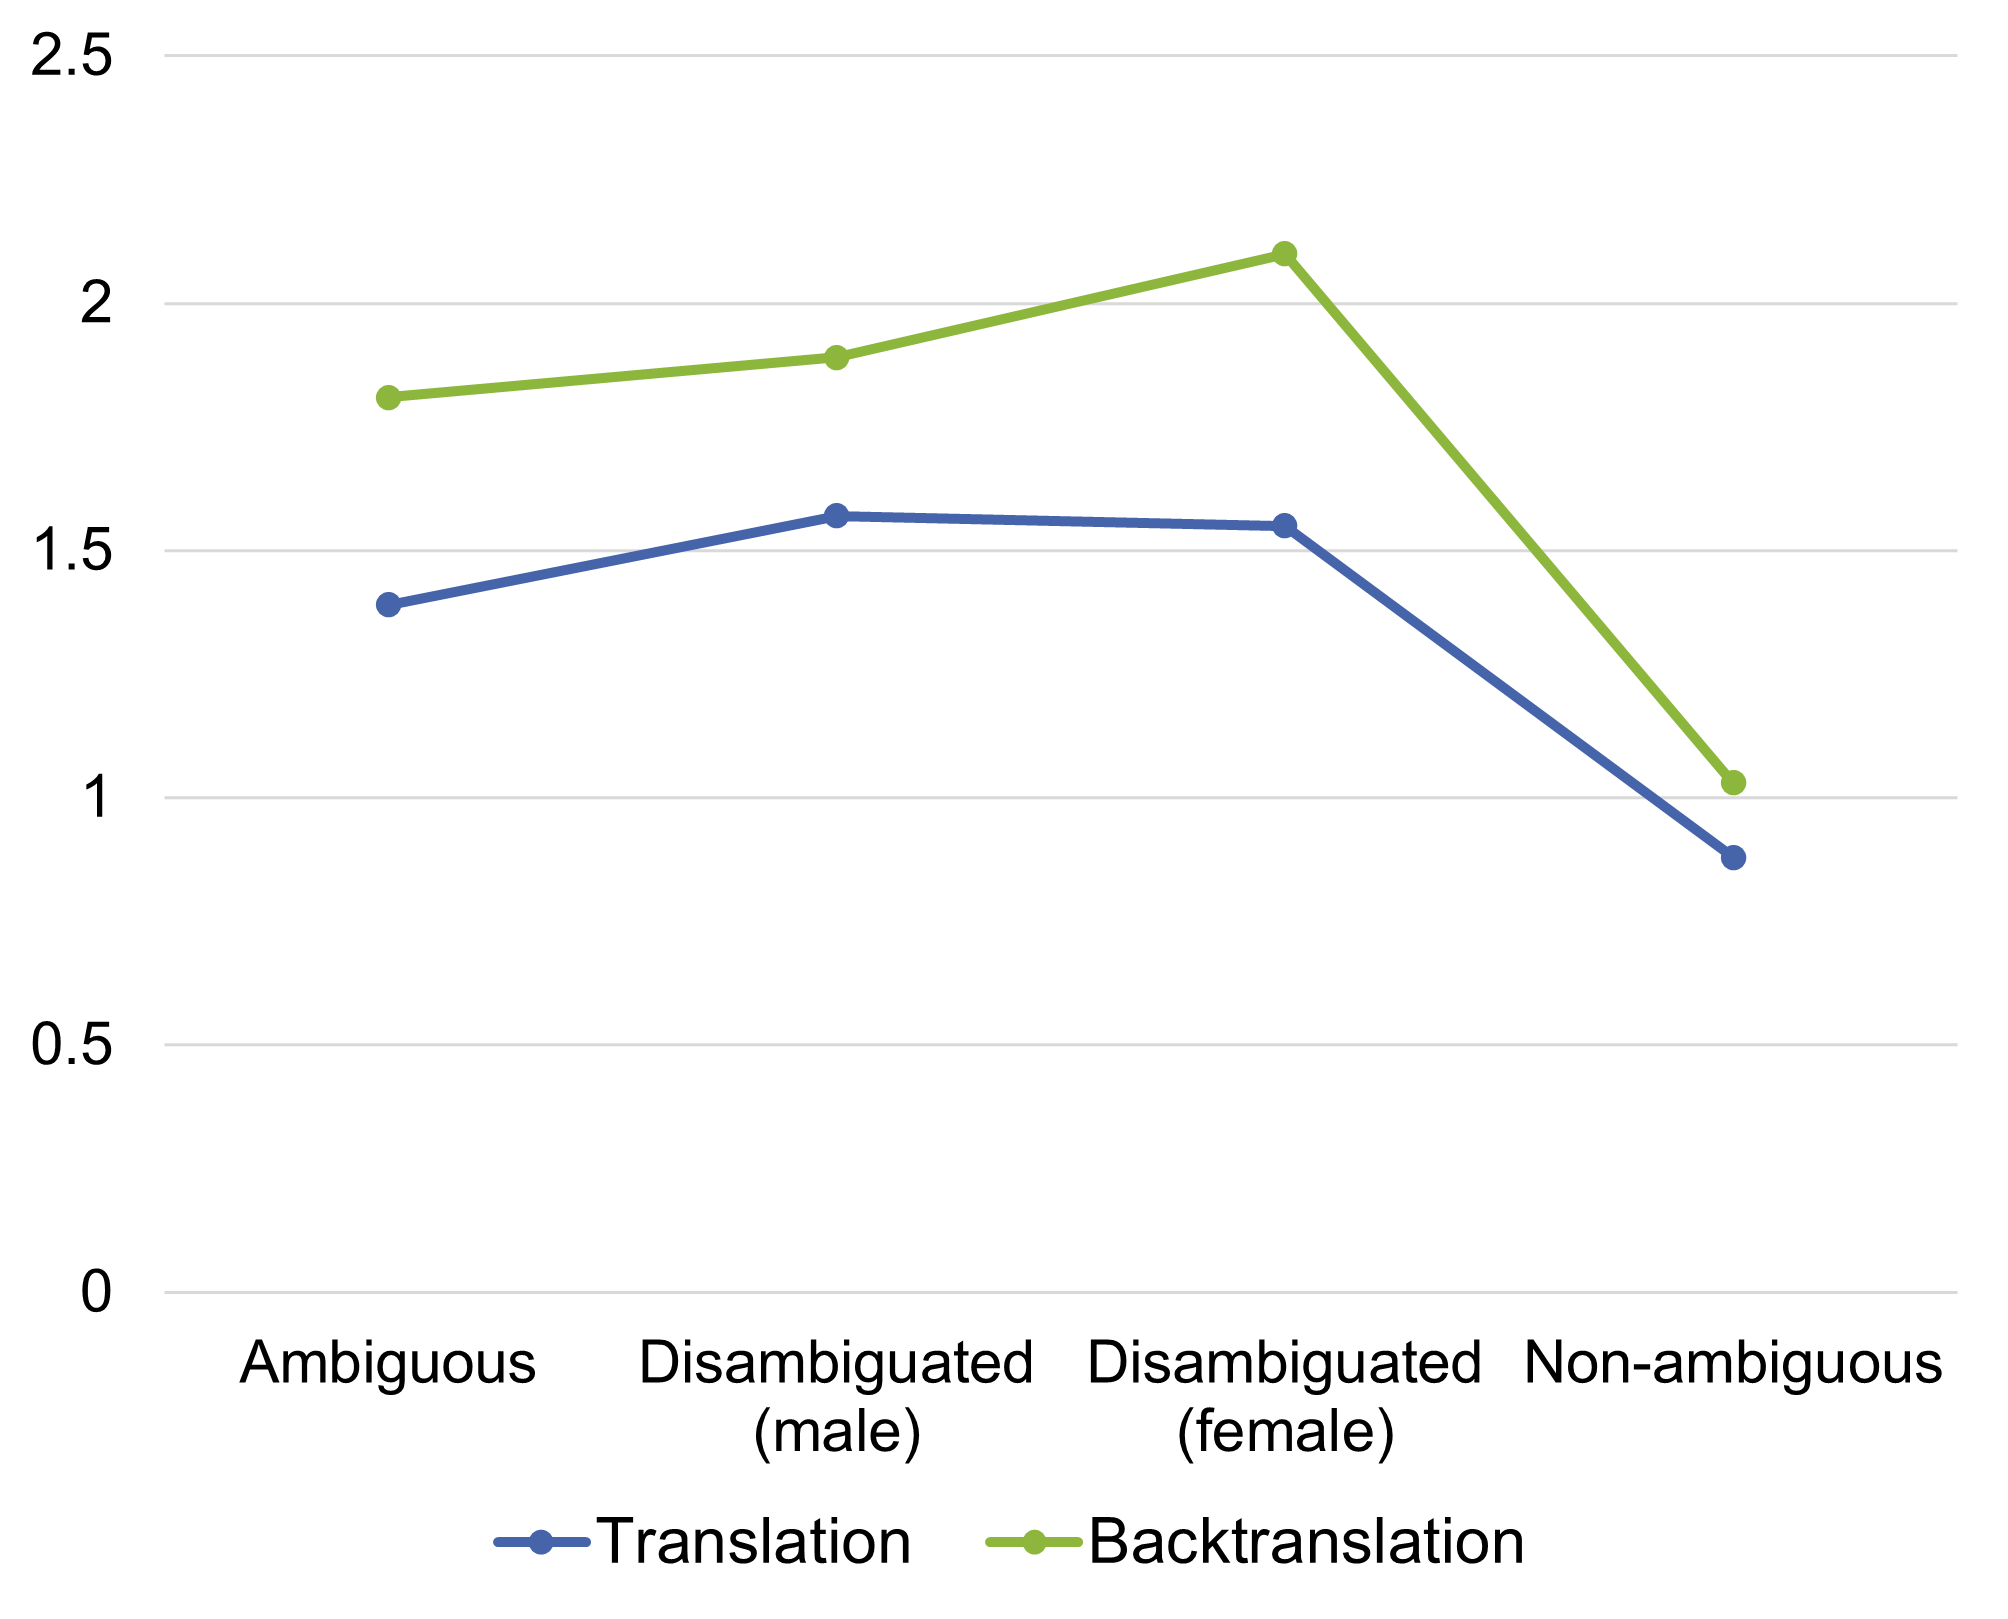
\includegraphics[width=\textwidth]{figures/correlation/words_beam10.png}
         \caption{Beam search with beam size 10}
         \label{fig:correlation_words_10}
     \end{subfigure}
     \hfill
     \begin{subfigure}{0.49\textwidth}
         \centering
         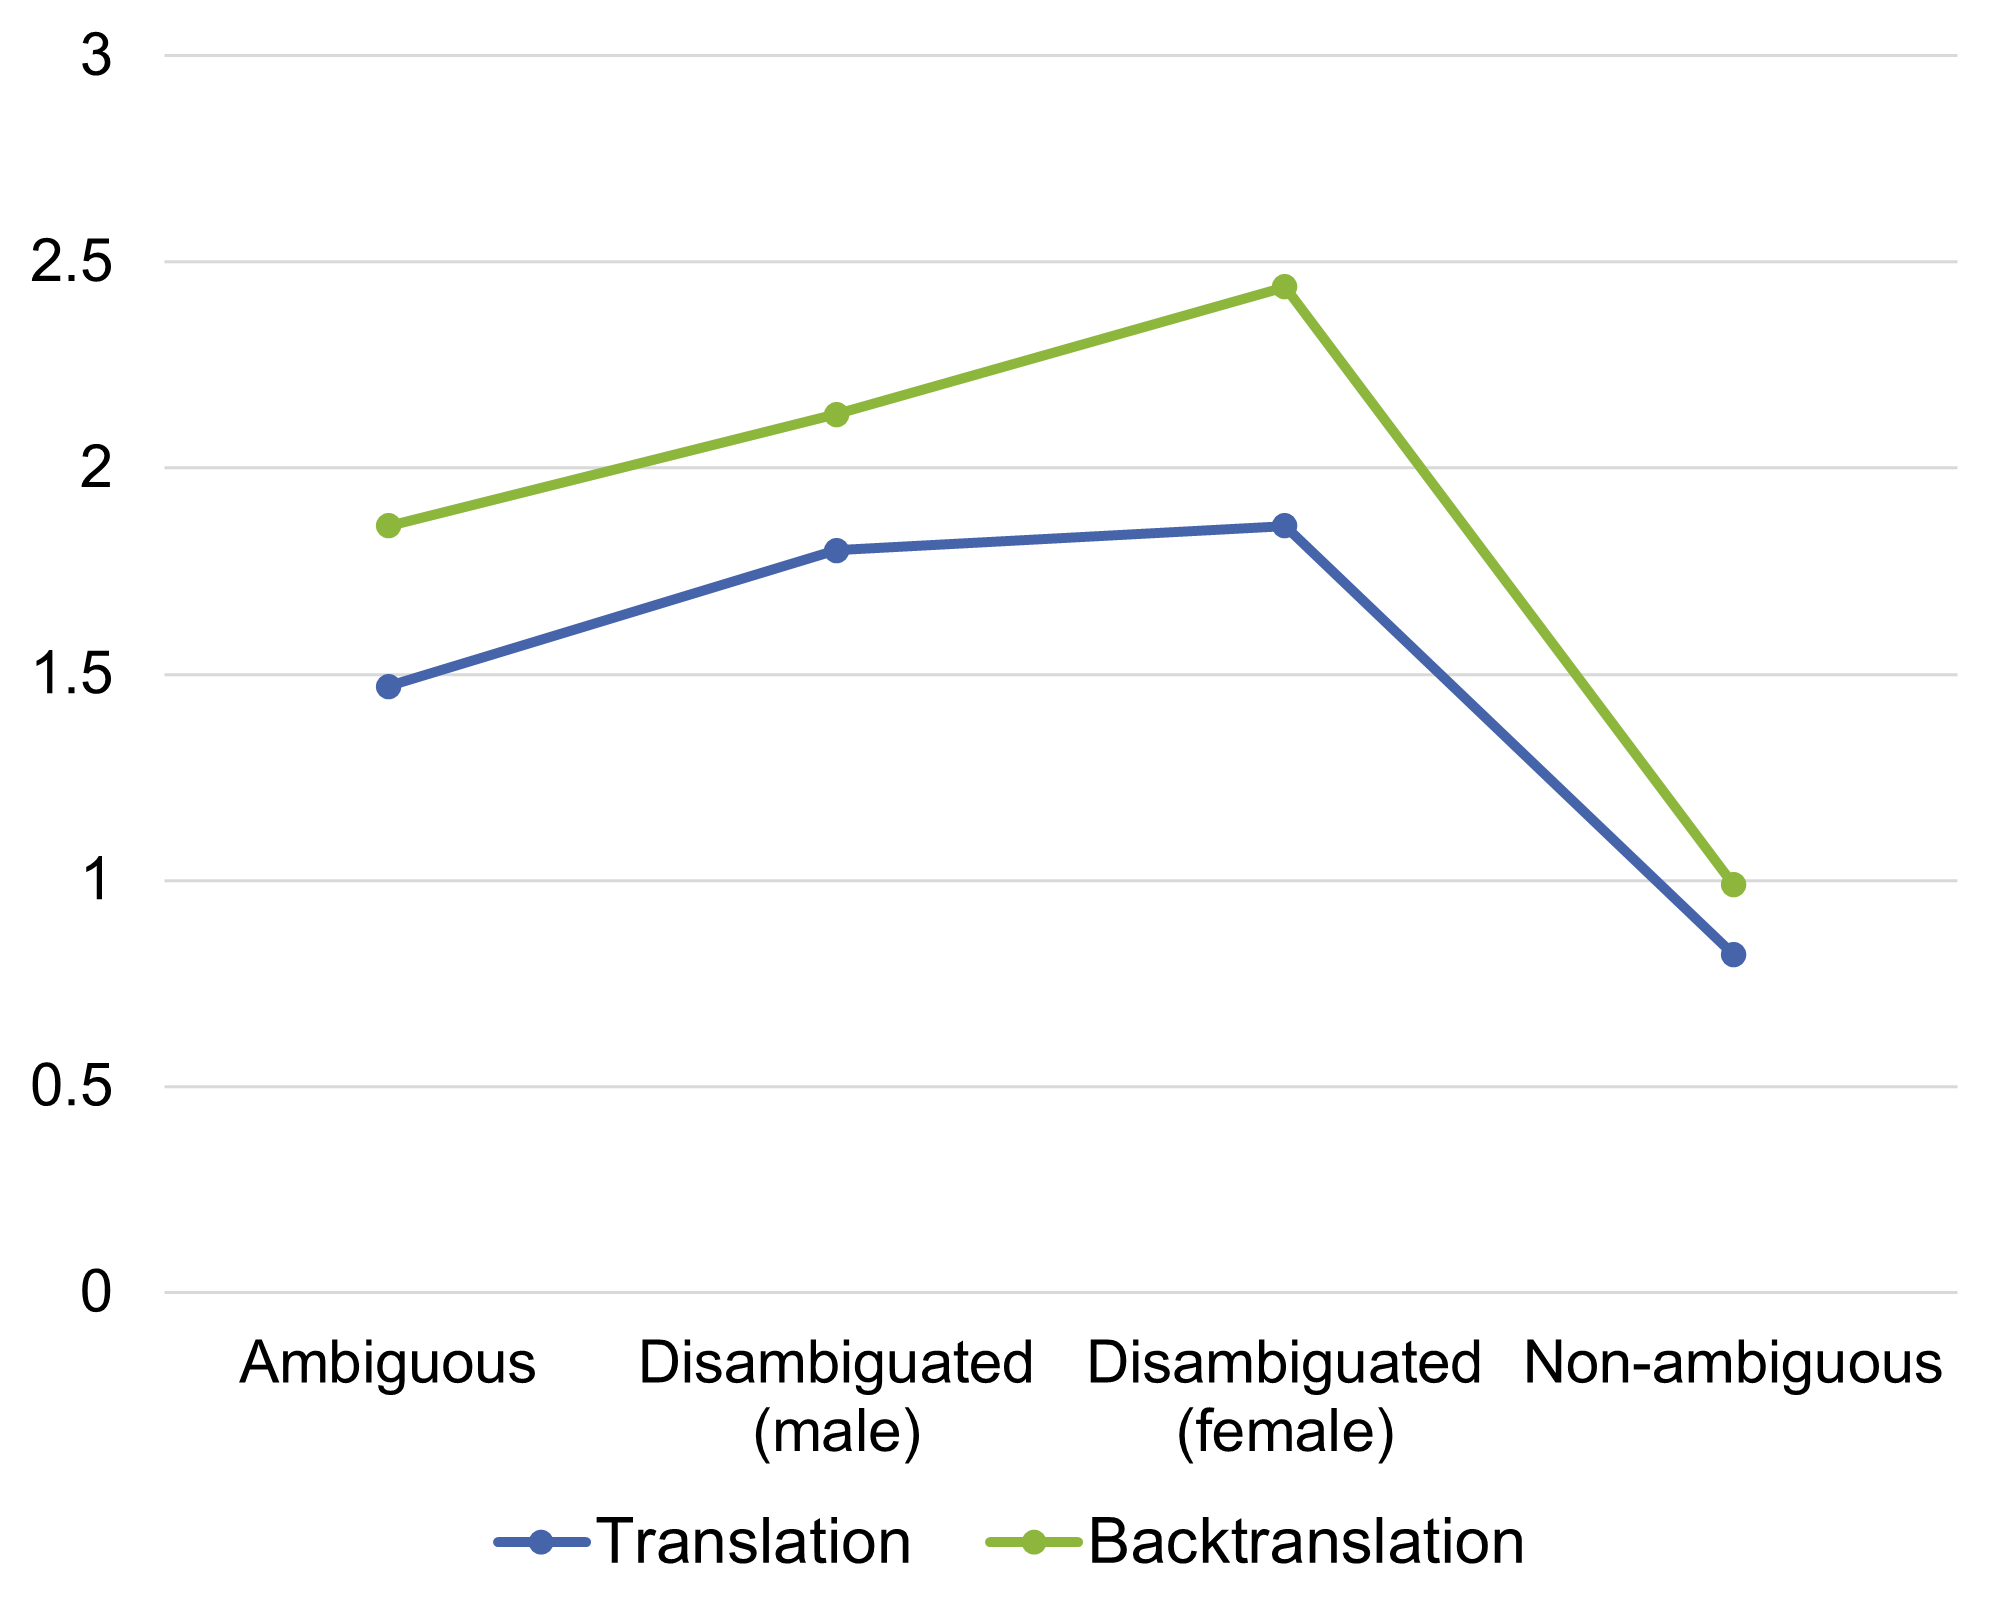
\includegraphics[width=\textwidth]{figures/correlation/words_sampling.png}
         \caption{Sampling}
         \label{fig:correlation_words_sampling}
     \end{subfigure}
     
    \caption{\textbf{Relationship Between Source Word and Rest of Sentence.} The results represent the amount of translations or backtranslations of the source word divided by the amount of translations or backtranslations of the rest of the sentence.}
    \label{fig:correlation_words}

\end{figure}